% Options for packages loaded elsewhere
\PassOptionsToPackage{unicode}{hyperref}
\PassOptionsToPackage{hyphens}{url}
%
\documentclass[
]{article}
\usepackage{lmodern}
\usepackage{amssymb,amsmath}
\usepackage{ifxetex,ifluatex}
\ifnum 0\ifxetex 1\fi\ifluatex 1\fi=0 % if pdftex
  \usepackage[T1]{fontenc}
  \usepackage[utf8]{inputenc}
  \usepackage{textcomp} % provide euro and other symbols
\else % if luatex or xetex
  \usepackage{unicode-math}
  \defaultfontfeatures{Scale=MatchLowercase}
  \defaultfontfeatures[\rmfamily]{Ligatures=TeX,Scale=1}
\fi
% Use upquote if available, for straight quotes in verbatim environments
\IfFileExists{upquote.sty}{\usepackage{upquote}}{}
\IfFileExists{microtype.sty}{% use microtype if available
  \usepackage[]{microtype}
  \UseMicrotypeSet[protrusion]{basicmath} % disable protrusion for tt fonts
}{}
\makeatletter
\@ifundefined{KOMAClassName}{% if non-KOMA class
  \IfFileExists{parskip.sty}{%
    \usepackage{parskip}
  }{% else
    \setlength{\parindent}{0pt}
    \setlength{\parskip}{6pt plus 2pt minus 1pt}}
}{% if KOMA class
  \KOMAoptions{parskip=half}}
\makeatother
\usepackage{xcolor}
\IfFileExists{xurl.sty}{\usepackage{xurl}}{} % add URL line breaks if available
\IfFileExists{bookmark.sty}{\usepackage{bookmark}}{\usepackage{hyperref}}
\hypersetup{
  pdftitle={Historical and Projected Water Balance Report for Crystal Bench},
  pdfauthor={Janelle Christensen, Mike Tercek, David Thoma, John Gross},
  hidelinks,
  pdfcreator={LaTeX via pandoc}}
\urlstyle{same} % disable monospaced font for URLs
\usepackage[margin=1in]{geometry}
\usepackage{graphicx,grffile}
\makeatletter
\def\maxwidth{\ifdim\Gin@nat@width>\linewidth\linewidth\else\Gin@nat@width\fi}
\def\maxheight{\ifdim\Gin@nat@height>\textheight\textheight\else\Gin@nat@height\fi}
\makeatother
% Scale images if necessary, so that they will not overflow the page
% margins by default, and it is still possible to overwrite the defaults
% using explicit options in \includegraphics[width, height, ...]{}
\setkeys{Gin}{width=\maxwidth,height=\maxheight,keepaspectratio}
% Set default figure placement to htbp
\makeatletter
\def\fps@figure{htbp}
\makeatother
\setlength{\emergencystretch}{3em} % prevent overfull lines
\providecommand{\tightlist}{%
  \setlength{\itemsep}{0pt}\setlength{\parskip}{0pt}}
\setcounter{secnumdepth}{-\maxdimen} % remove section numbering

\title{Historical and Projected Water Balance Report for Crystal Bench}
\author{Janelle Christensen, Mike Tercek, David Thoma, John Gross}
\date{8/3/2020}

\begin{document}
\maketitle

Water balance is the mathematical accounting of water input and movement
through the environment. It accounts for water storage in different
phases (ice, liquid) and loss to the atmosphere (gas) via
evapotranspiration. Water balance integrates the interactions of
temperature and precipitation to estimate water availability, movement
to streams and ground water and use by plants. Water balance accounts
for heat load on different aspects and water holding capacity of
different soil types. Water balance represents the modification of
regional weather and climate to represent the biophysical conditions at
local scales. For these reasons, water balance is usually more strongly
correlated with natural resource response (plant growth, stream flow,
fire danger) than temperature or precipitation.

\begin{center}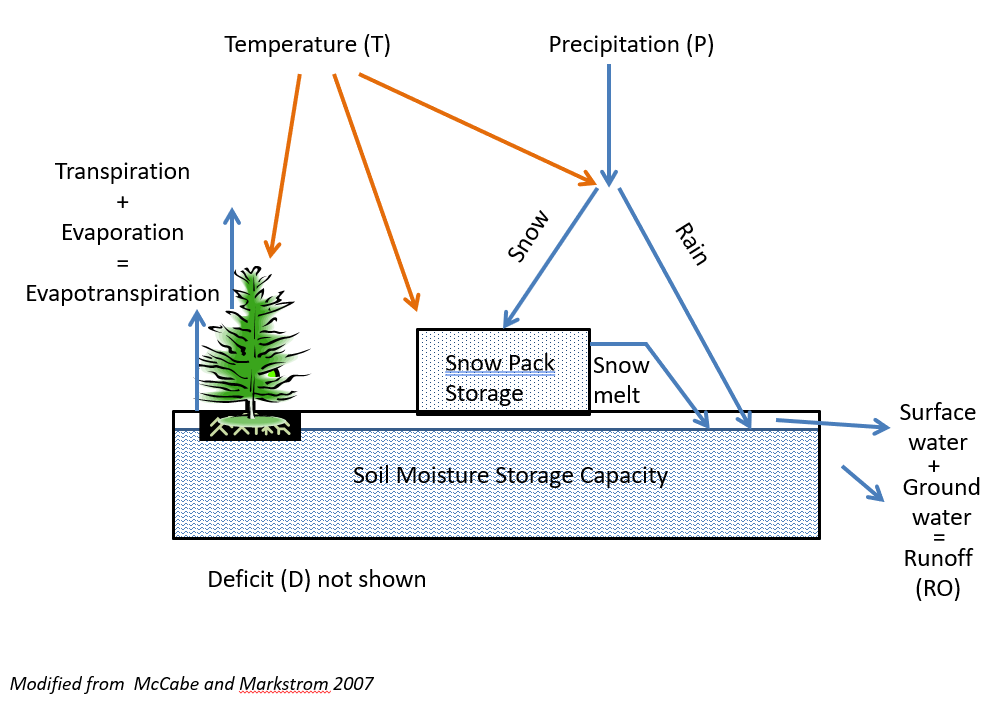
\includegraphics[width=0.6\linewidth]{C:/Users/jnchr/Documents/R/Water Balance/figures/mccabe_and_markstrom} \end{center}

This report is created from temperature and precipitation data that is
input to a water balance model. The historical temperature and
precipitation data are from
\href{http://www.climatologylab.org/gridmet.html}{gridMET}. The future
climate projections, inmcm4 RCP 4.5 and HadGEM2-CC365 RCP 8.5, are from
the \href{https://www.wcrp-climate.org/wgcm-cmip/wgcm-cmip5}{CMIP5
experiments} . The water balance model is maintained by the National
Park Service (Mike Tercek, David Thoma and John Gross). Collectively
this report summarizes historical and projected biophysical
environmental conditions from 1980-2100 at the single grid cell level
(gridMET = 4km; projections = 1km). A link to the NPS water balance
gridded products an be found
\href{http://www.yellowstone.solutions/thredds/catalog.html}{here}.

\hypertarget{selection-of-the-models}{%
\subsection{Selection of the Models}\label{selection-of-the-models}}

The models used in this analysis were chosen based upon which two
climate futures best bracket the range of possibilities. For this
region, the model selection was based off of the latitude and longitude
for each park centroid, plotted on the scatterplot visualization of
future projections from the
\href{https://climate.northwestknowledge.net/MACA/vis_scatterplot.php}{MACA
website.}. Models were selected to represent a ``drier and hotter''
climate future (the bottom right of the scatterplot) and a ``wetter and
hotter'' climate future (the upper left of the scatterplot).

\hypertarget{annual-values-through-time}{%
\subsection{Annual values through
time}\label{annual-values-through-time}}

The variables of runoff, rain, potential evapotranspiration (PET),
actual evapotranspiration (AET), and deficit are summed to show annual
values through time. Accumulated snow water equivalent (SWE) shows the
max value for the year regardless of the month it occurs in. Accumulated
growing degree days (AGDD) starts accumulating on October 1 of the
previous year, and the max value is taken at its highest point. Soil
water shows the mean value for the year.

The reason for the different summary statistics is because hydrologist
use these variables in different ways. Water variables that don't have
an upper limit like rain, runoff, evapostranspiration and deficit can
accumulate indefinitely within a calendar year, whereas soil moisture is
limited by the soil water holding capacity so it is averaged on an
annual basis. Temperature variables are averaged by convention and
growing degree days are summed to account for the seasonal accumulation
of heat that controls biological metabolism and thus growth rates and
phenology when water is available. For the variables that are
accumulated, we take the max of the variable because it is already a
summation of the total through the year.

\begin{figure}

{\centering 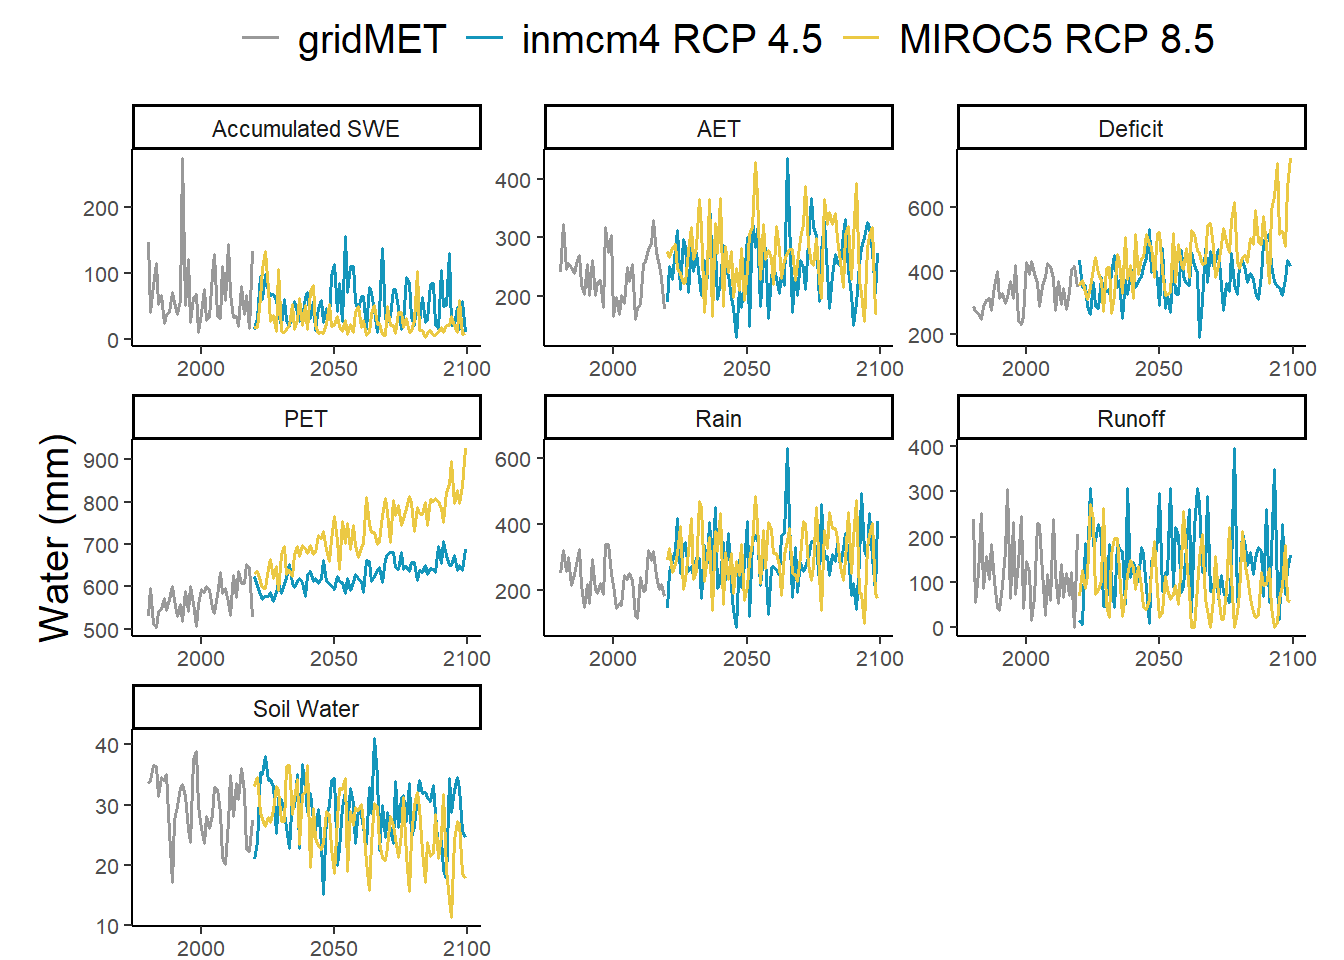
\includegraphics{water_balance_graphs_files/figure-latex/unnamed-chunk-18-1} 

}

\caption{Figure 1. Annual averages over time. The gray line represents historical data modeled from gridMET climate data, the turquoise line represents inmcm4 rcp45 and the yellow line represents HadGEM2-CC365 rcp85}\label{fig:unnamed-chunk-18}
\end{figure}

\hypertarget{deficit-v.-actual-evapotranspiration-aet}{%
\subsection{Deficit v. Actual Evapotranspiration
(AET)}\label{deficit-v.-actual-evapotranspiration-aet}}

Deficit (D) and actual evapotranspiration (AET) represent unmet water
needs of vegetation and vegetation water use. They are good predictors
of vegetation type, and are useful variables in understanding climate
stress on vegetation and how vegetation may transition in the future
(Stephenson, 1998). If the clustering of AET and deficit change in
climate space, vegetation assemblages will respond and changes in
assemblages will eventually reflect the new climate space. The figure
below (from Stephenson) shows how AET v. D differs across bioregions in
the U.S.

\begin{figure}

{\centering 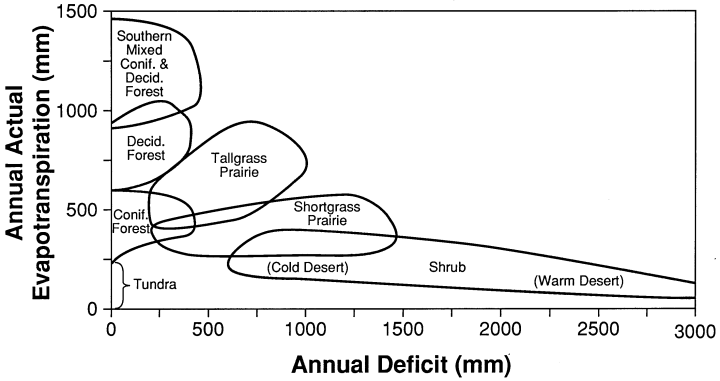
\includegraphics[width=0.5\linewidth]{C:/Users/jnchr/Documents/R/Water Balance/figures/aet_v_d} 

}

\caption{Figure 2. Stephenson (1998)}\label{fig:unnamed-chunk-19}
\end{figure}

\begin{figure}
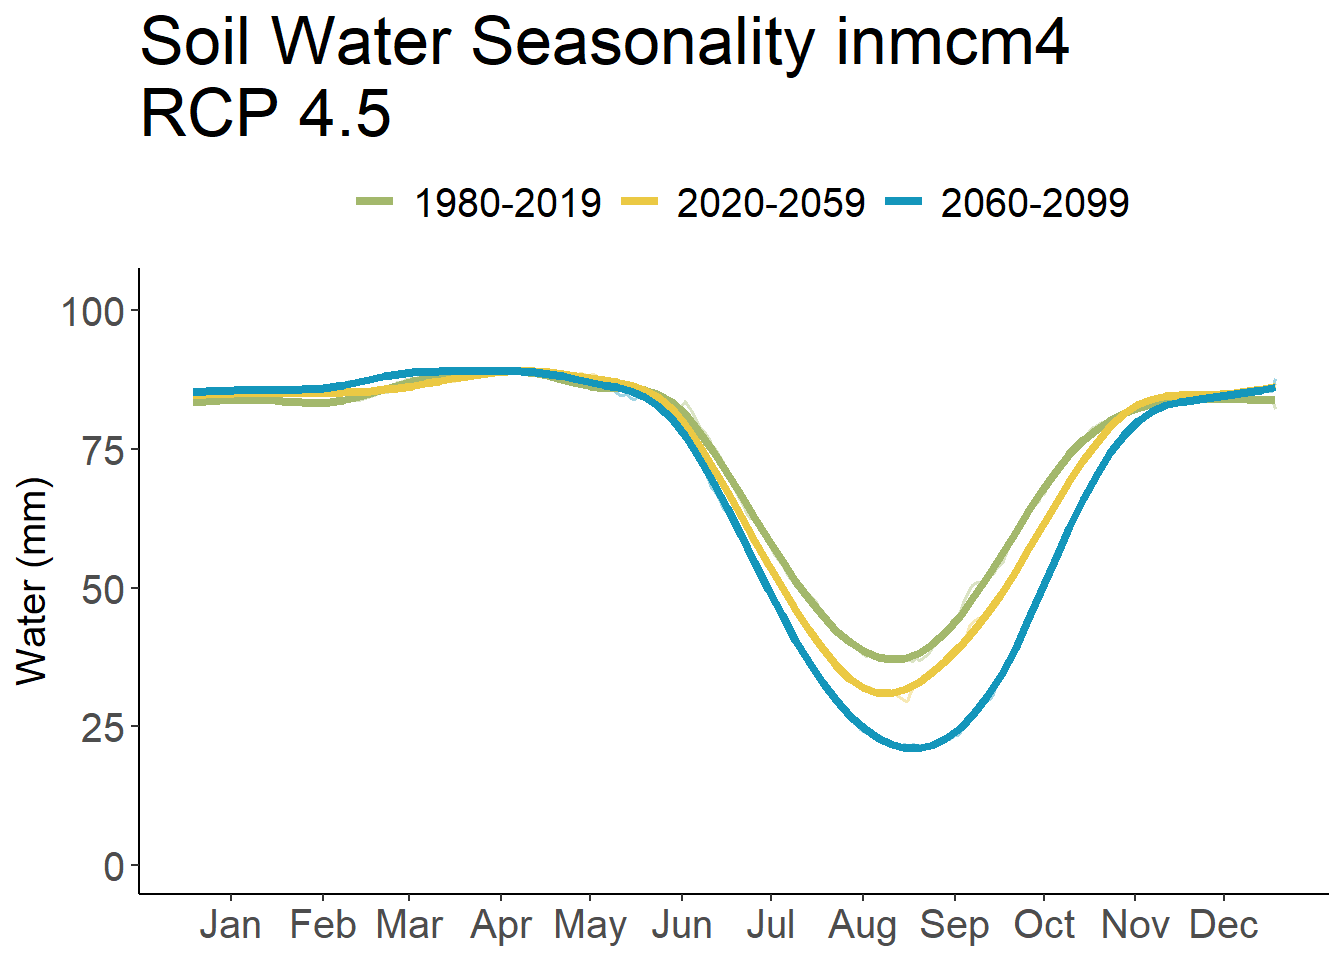
\includegraphics[width=0.5\linewidth]{water_balance_graphs_files/figure-latex/unnamed-chunk-20-1} 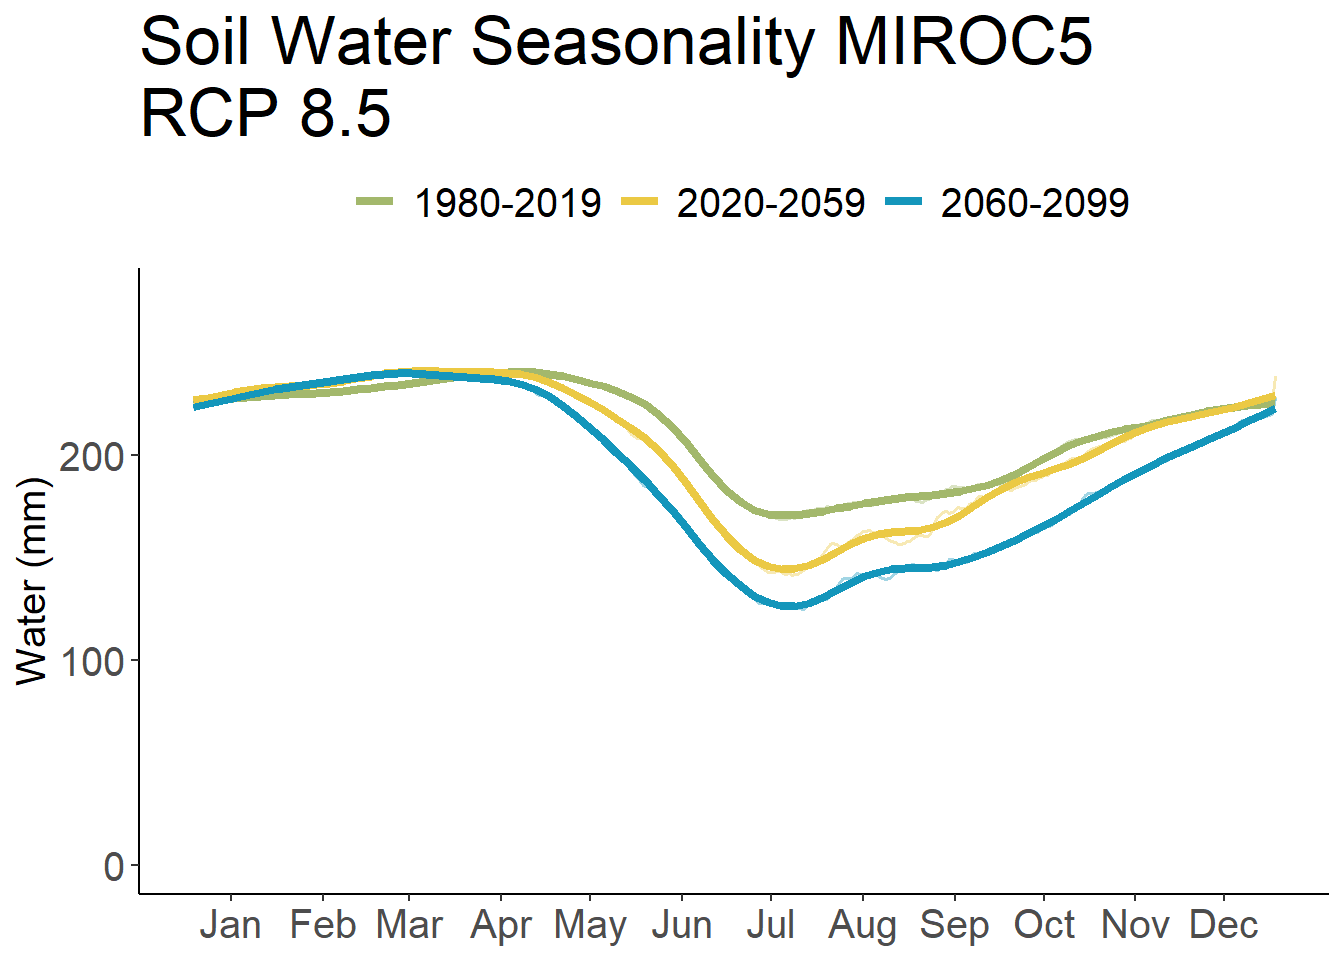
\includegraphics[width=0.5\linewidth]{water_balance_graphs_files/figure-latex/unnamed-chunk-20-2} \caption{Figure 3. Modeled Deficit vs. AET. The points are annual sums of daily observations in each year. The green points represent 1980-2019; the yellow points 2020-2059; and the turquoise points 2060-2099. The contours around each set of points encircle the climate space for inmcm4 rcp45 and HadGEM2-CC365 rcp85.}\label{fig:unnamed-chunk-20}
\end{figure}

\hypertarget{soil-water}{%
\subsection{Soil Water}\label{soil-water}}

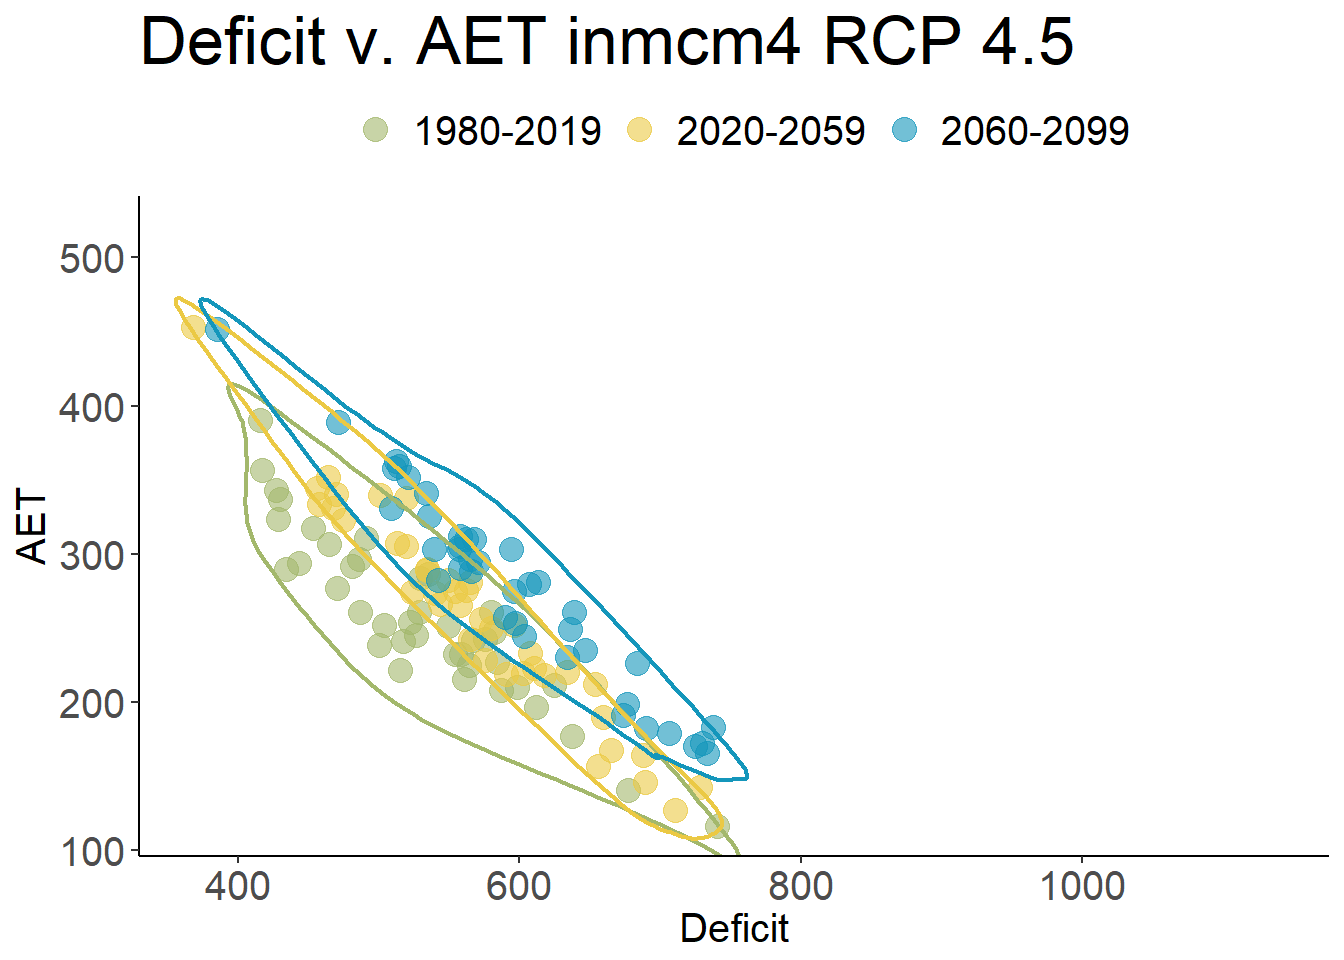
\includegraphics[width=0.5\linewidth]{water_balance_graphs_files/figure-latex/unnamed-chunk-21-1}
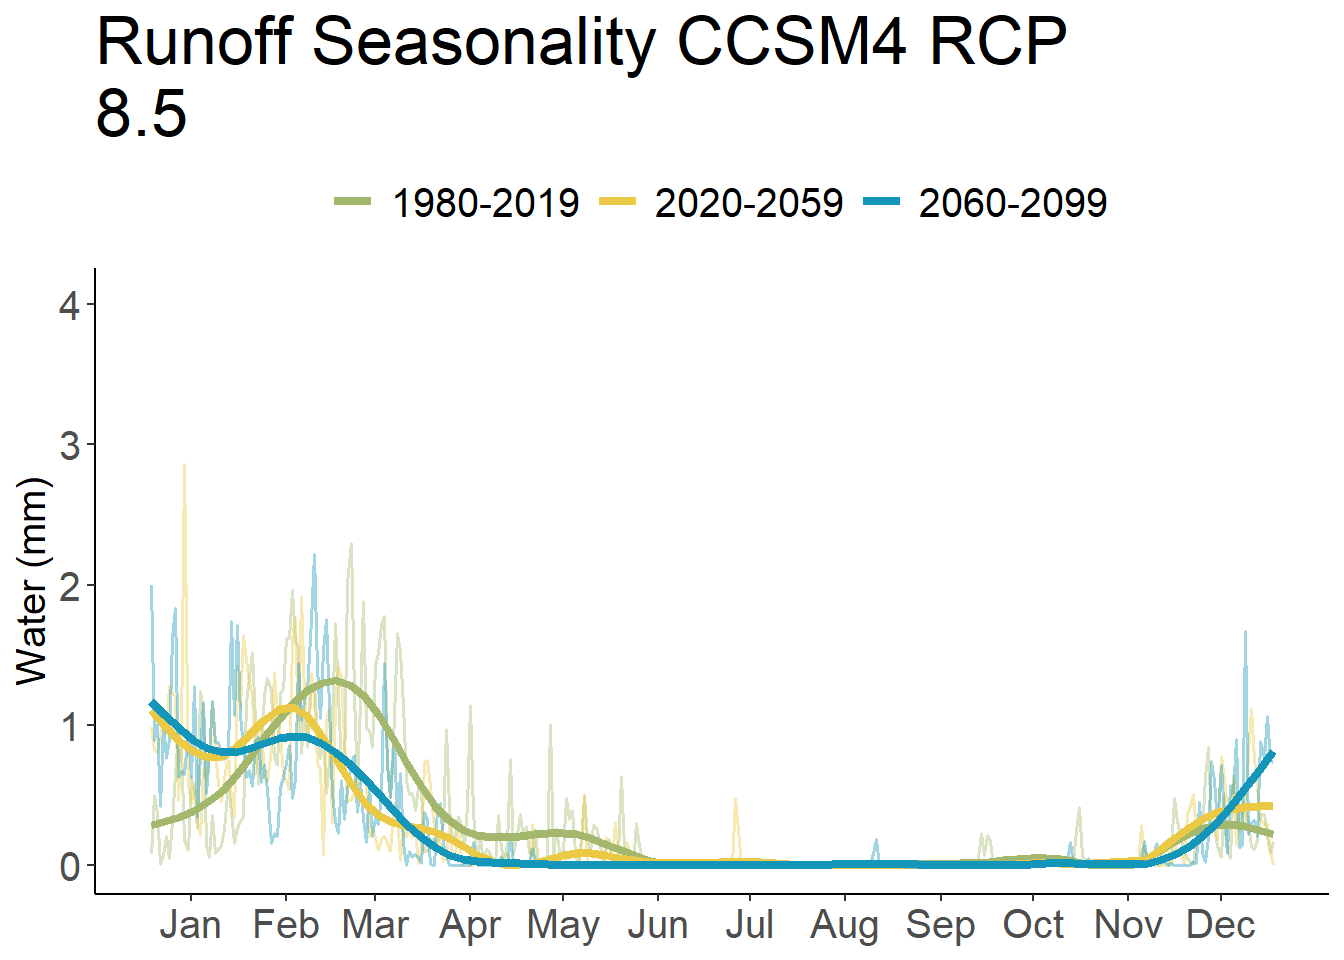
\includegraphics[width=0.5\linewidth]{water_balance_graphs_files/figure-latex/unnamed-chunk-21-2}
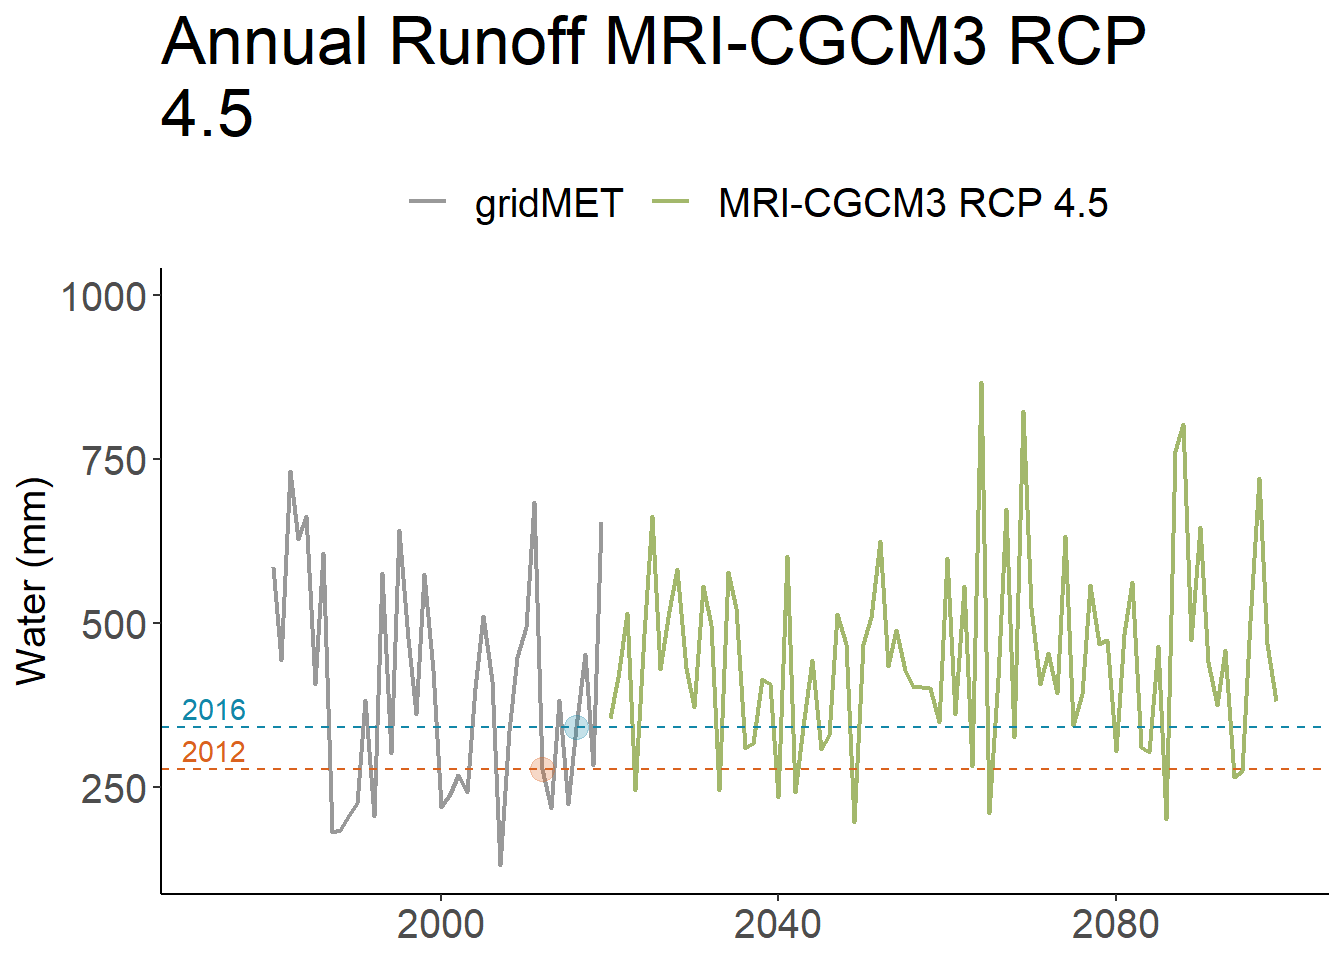
\includegraphics[width=0.5\linewidth]{water_balance_graphs_files/figure-latex/unnamed-chunk-21-3}
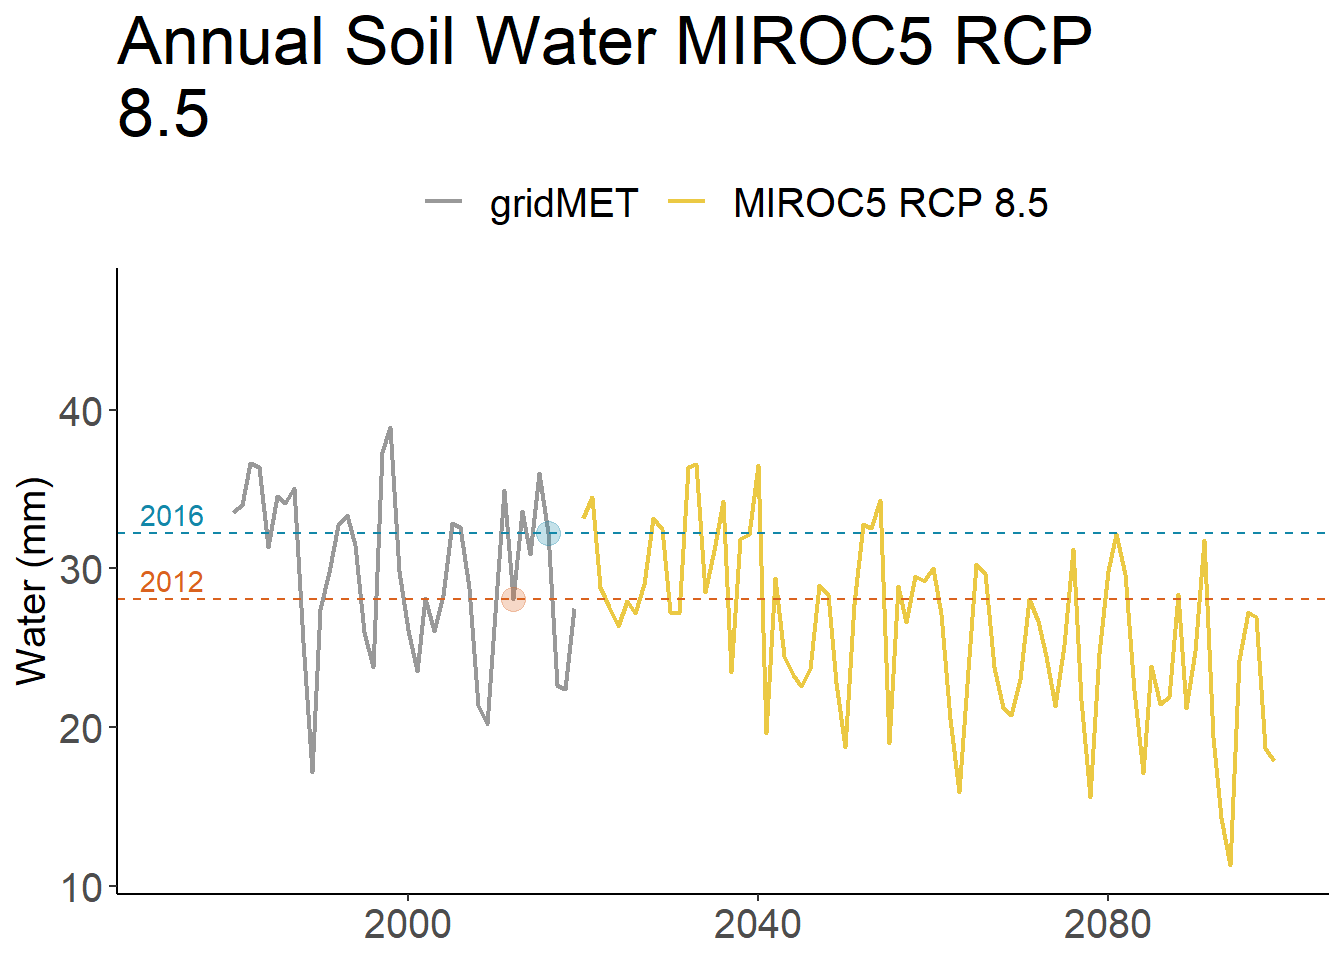
\includegraphics[width=0.5\linewidth]{water_balance_graphs_files/figure-latex/unnamed-chunk-21-4}
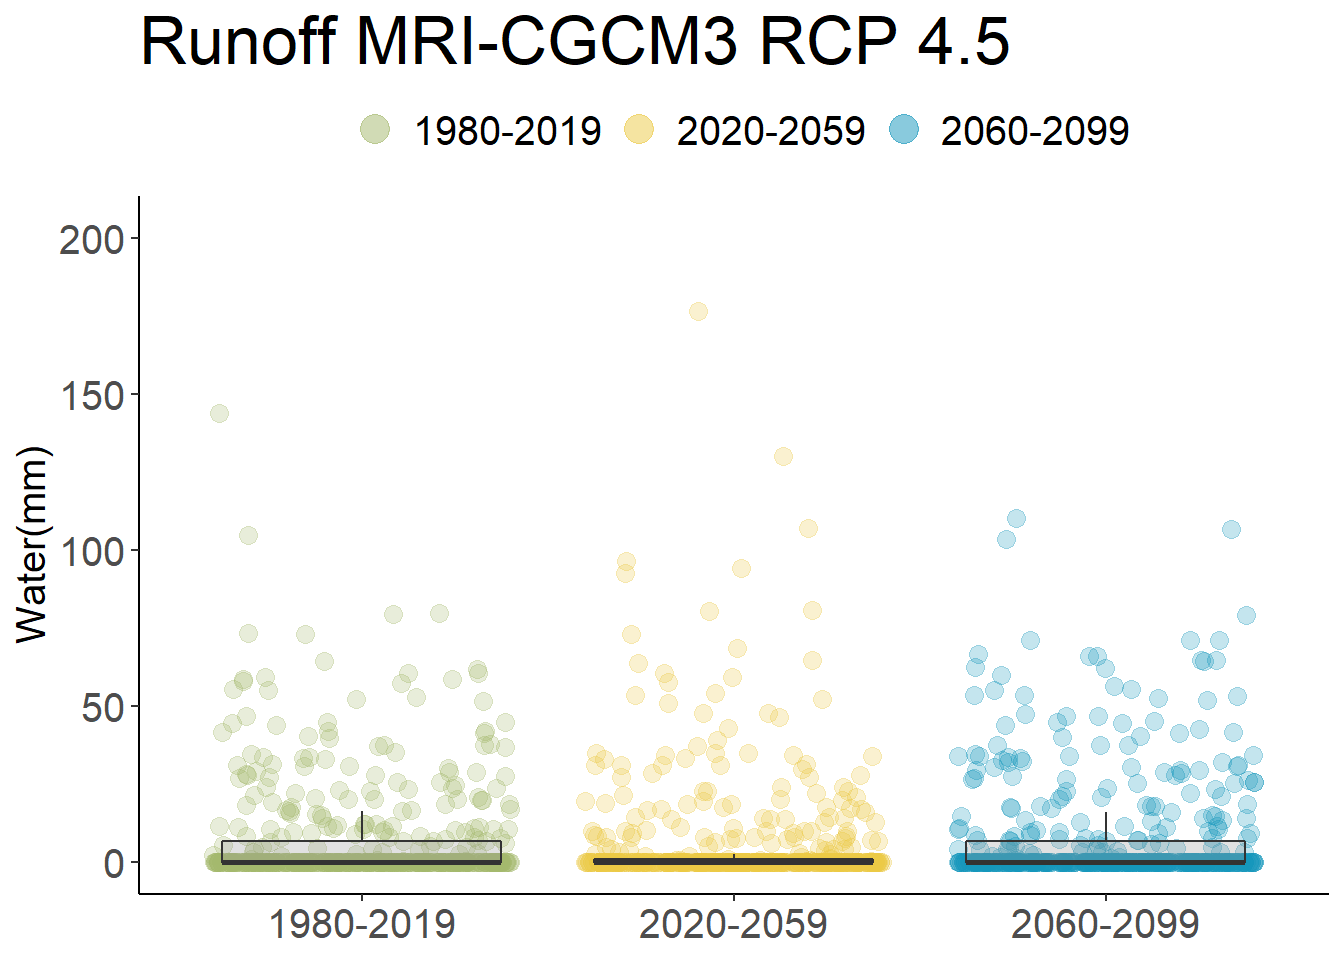
\includegraphics[width=0.5\linewidth]{water_balance_graphs_files/figure-latex/unnamed-chunk-21-5}
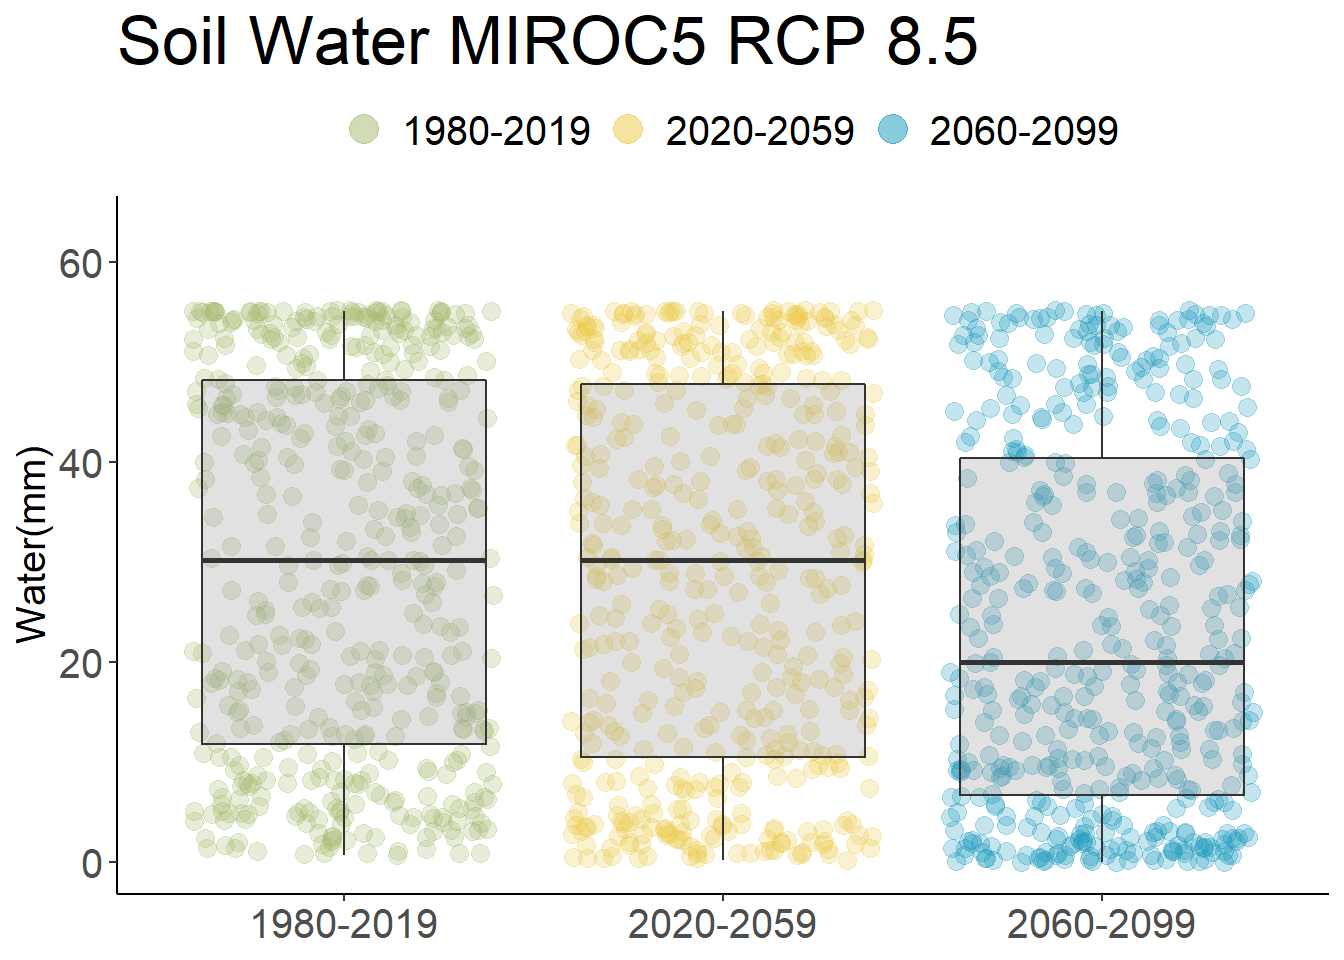
\includegraphics[width=0.5\linewidth]{water_balance_graphs_files/figure-latex/unnamed-chunk-21-6}

\hypertarget{runoff}{%
\subsection{Runoff}\label{runoff}}

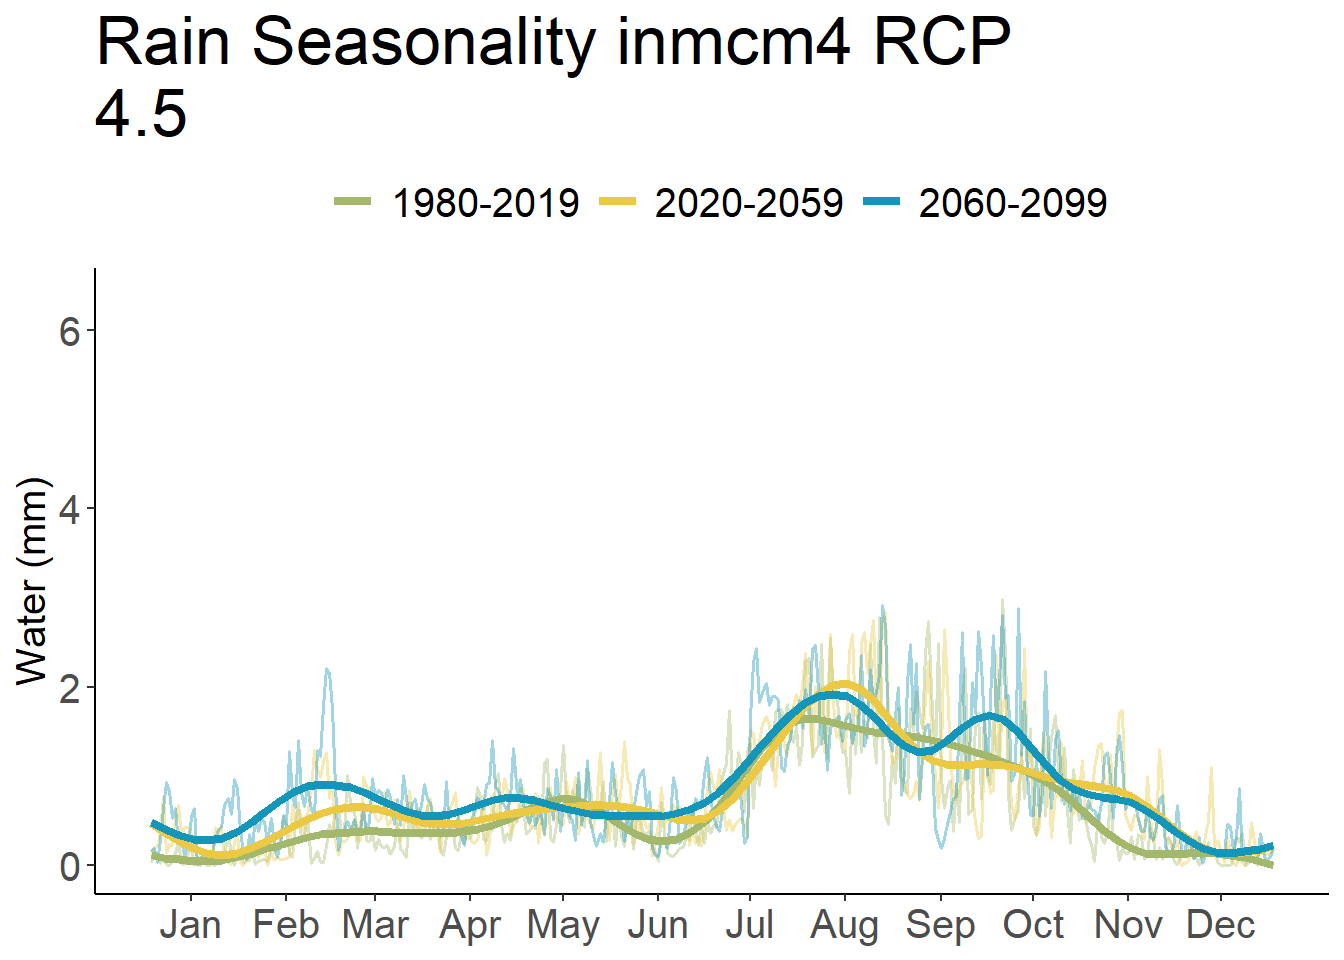
\includegraphics[width=0.5\linewidth]{water_balance_graphs_files/figure-latex/unnamed-chunk-22-1}
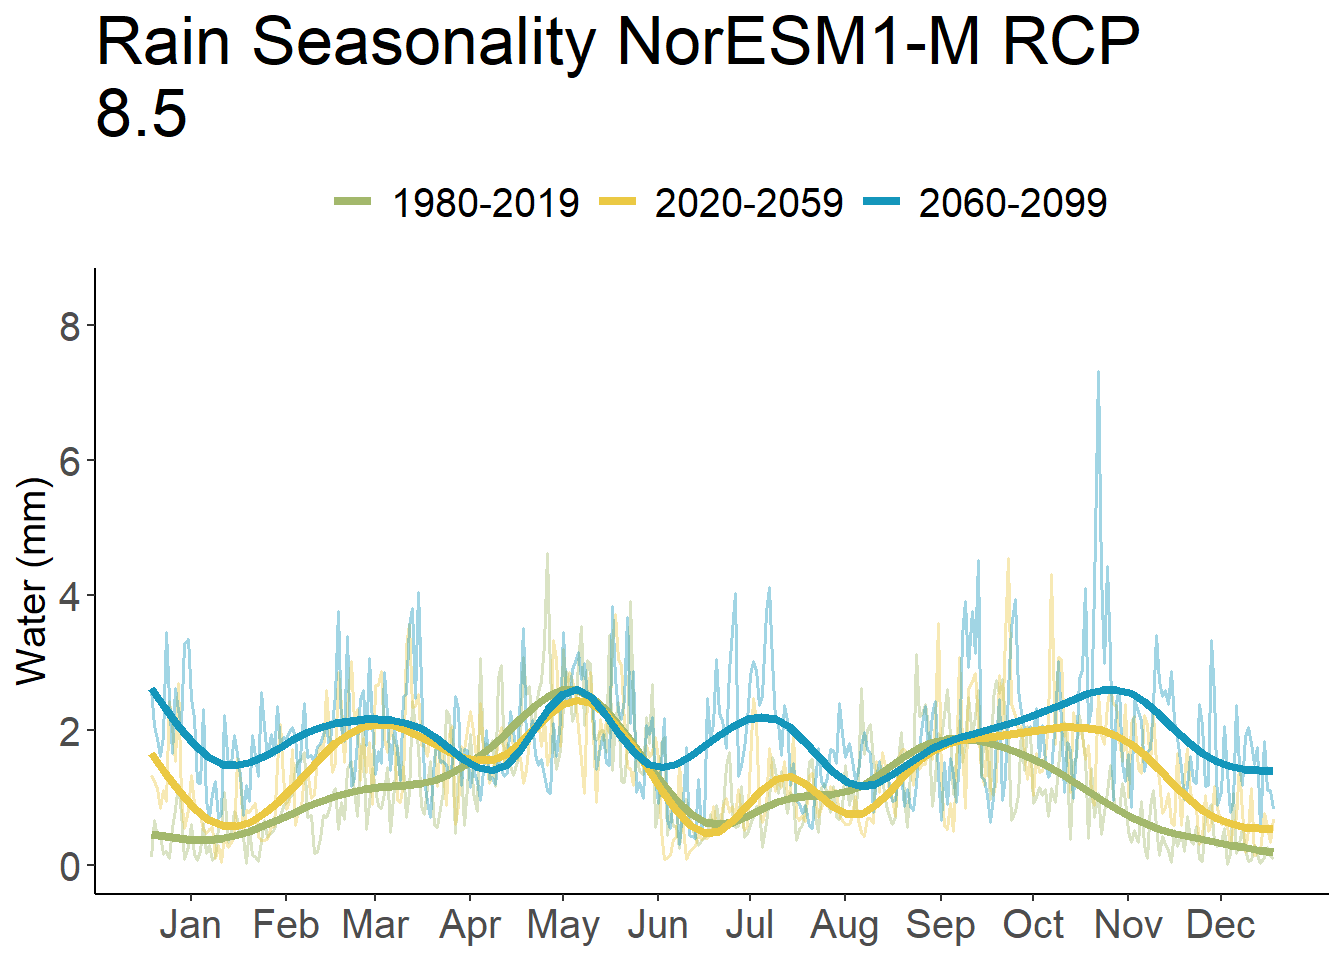
\includegraphics[width=0.5\linewidth]{water_balance_graphs_files/figure-latex/unnamed-chunk-22-2}
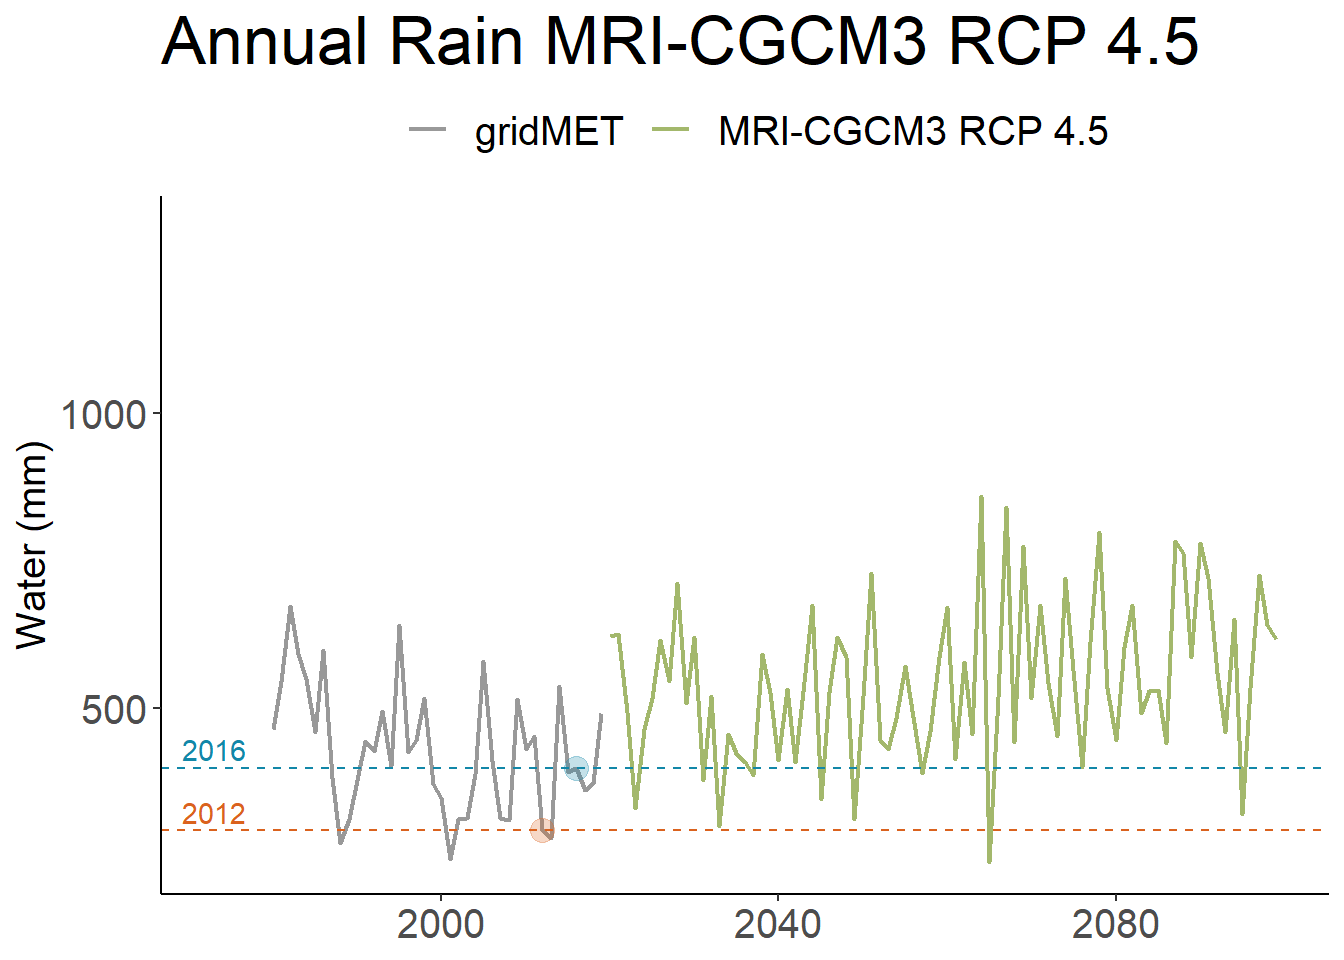
\includegraphics[width=0.5\linewidth]{water_balance_graphs_files/figure-latex/unnamed-chunk-22-3}
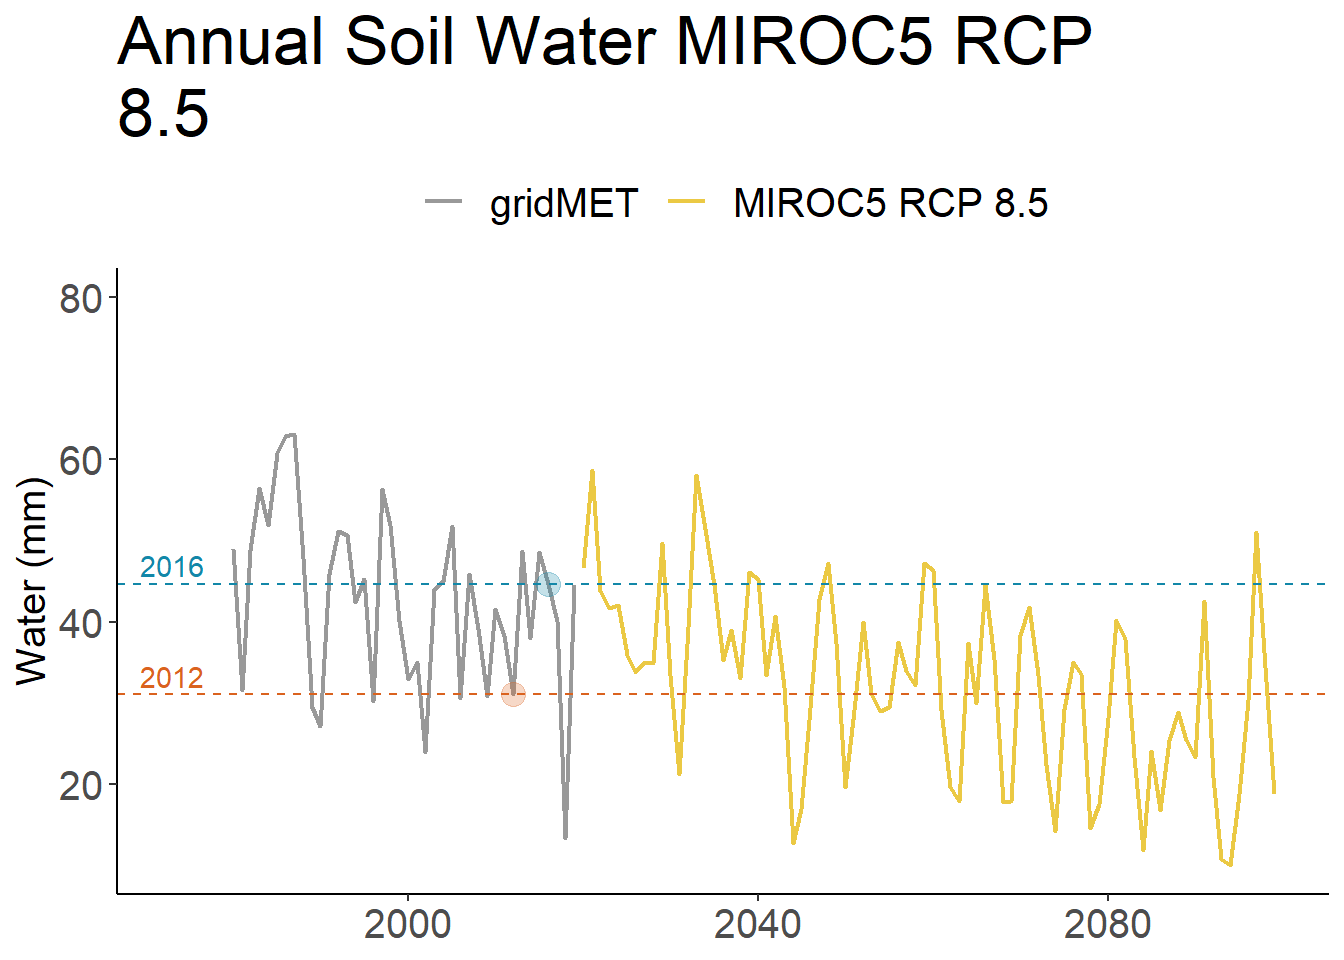
\includegraphics[width=0.5\linewidth]{water_balance_graphs_files/figure-latex/unnamed-chunk-22-4}
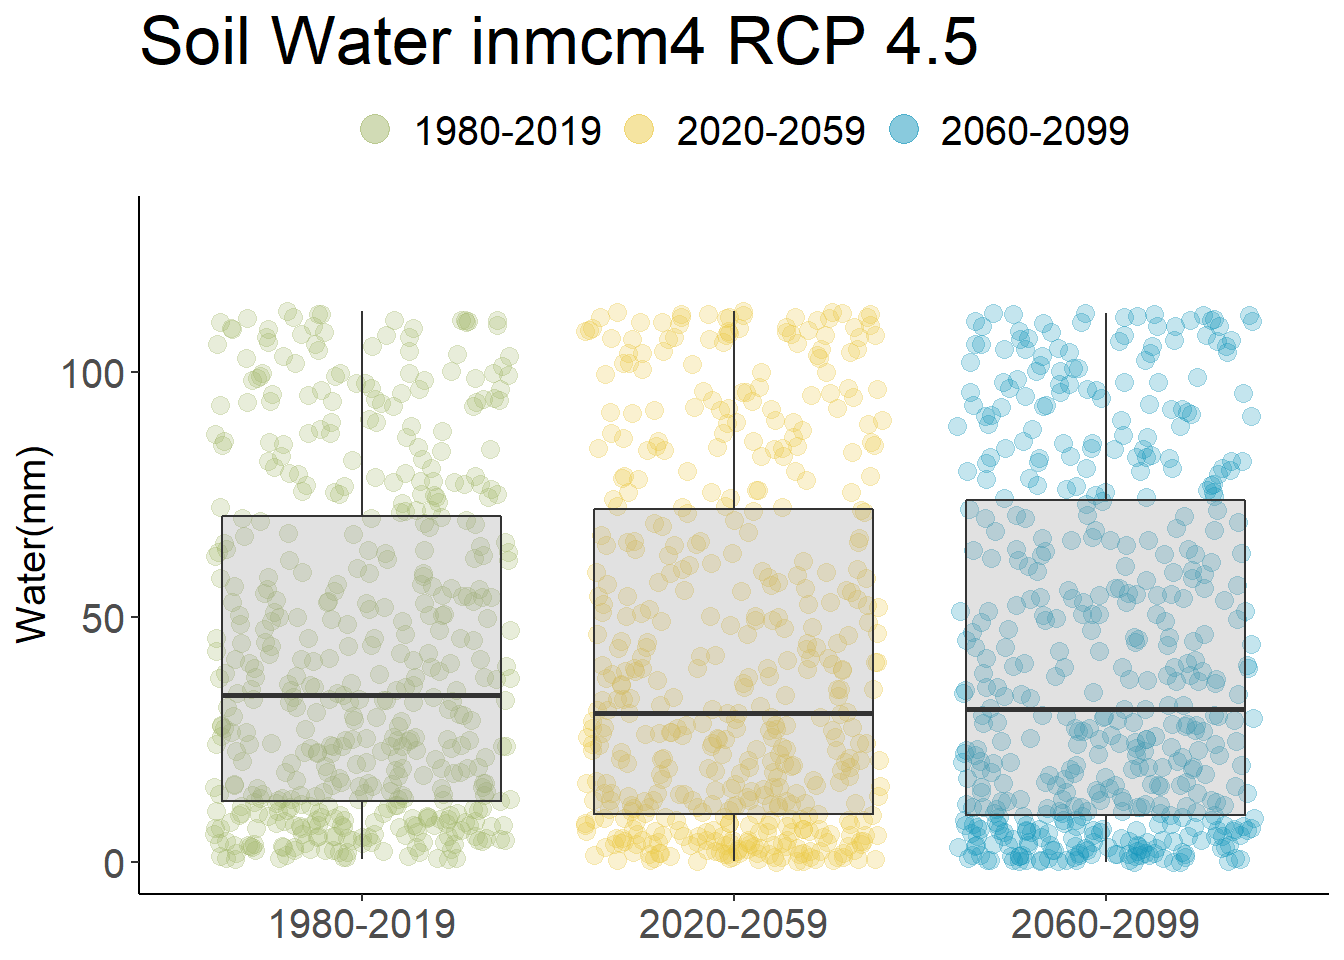
\includegraphics[width=0.5\linewidth]{water_balance_graphs_files/figure-latex/unnamed-chunk-22-5}
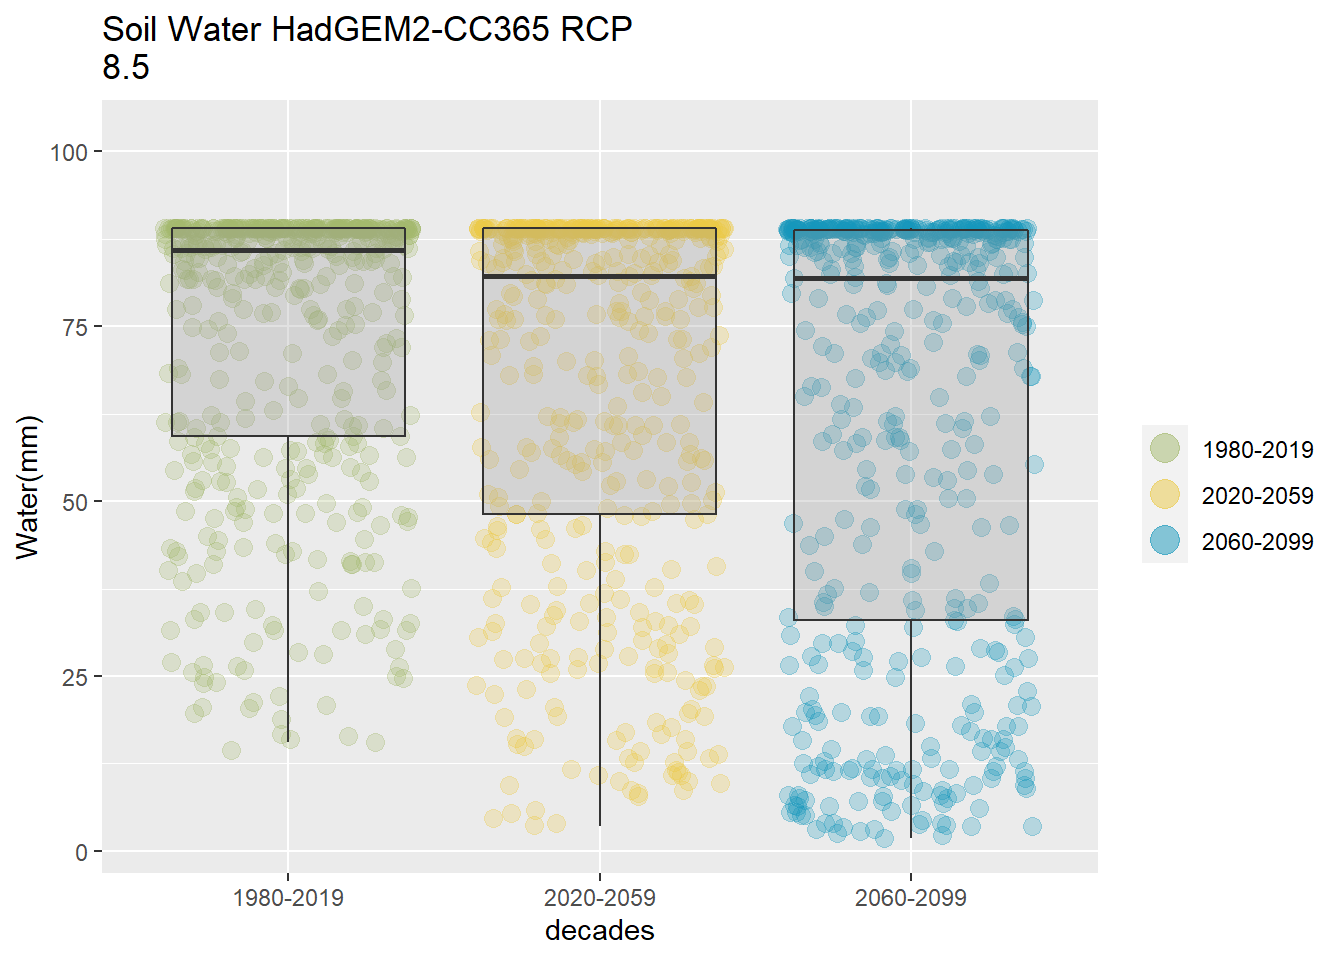
\includegraphics[width=0.5\linewidth]{water_balance_graphs_files/figure-latex/unnamed-chunk-22-6}

\hypertarget{rain}{%
\subsection{Rain}\label{rain}}

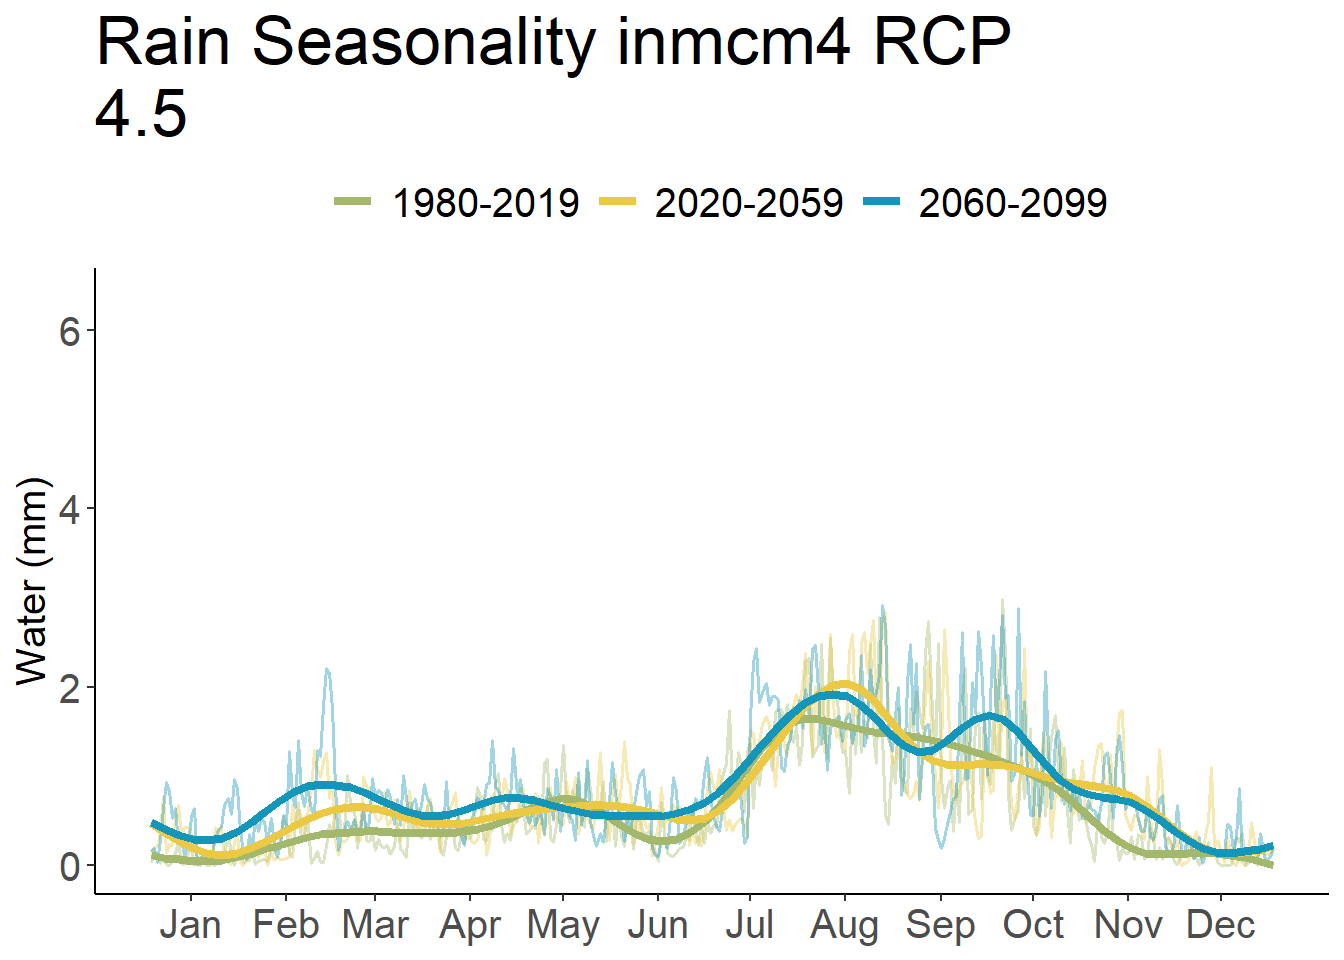
\includegraphics[width=0.5\linewidth]{water_balance_graphs_files/figure-latex/unnamed-chunk-23-1}
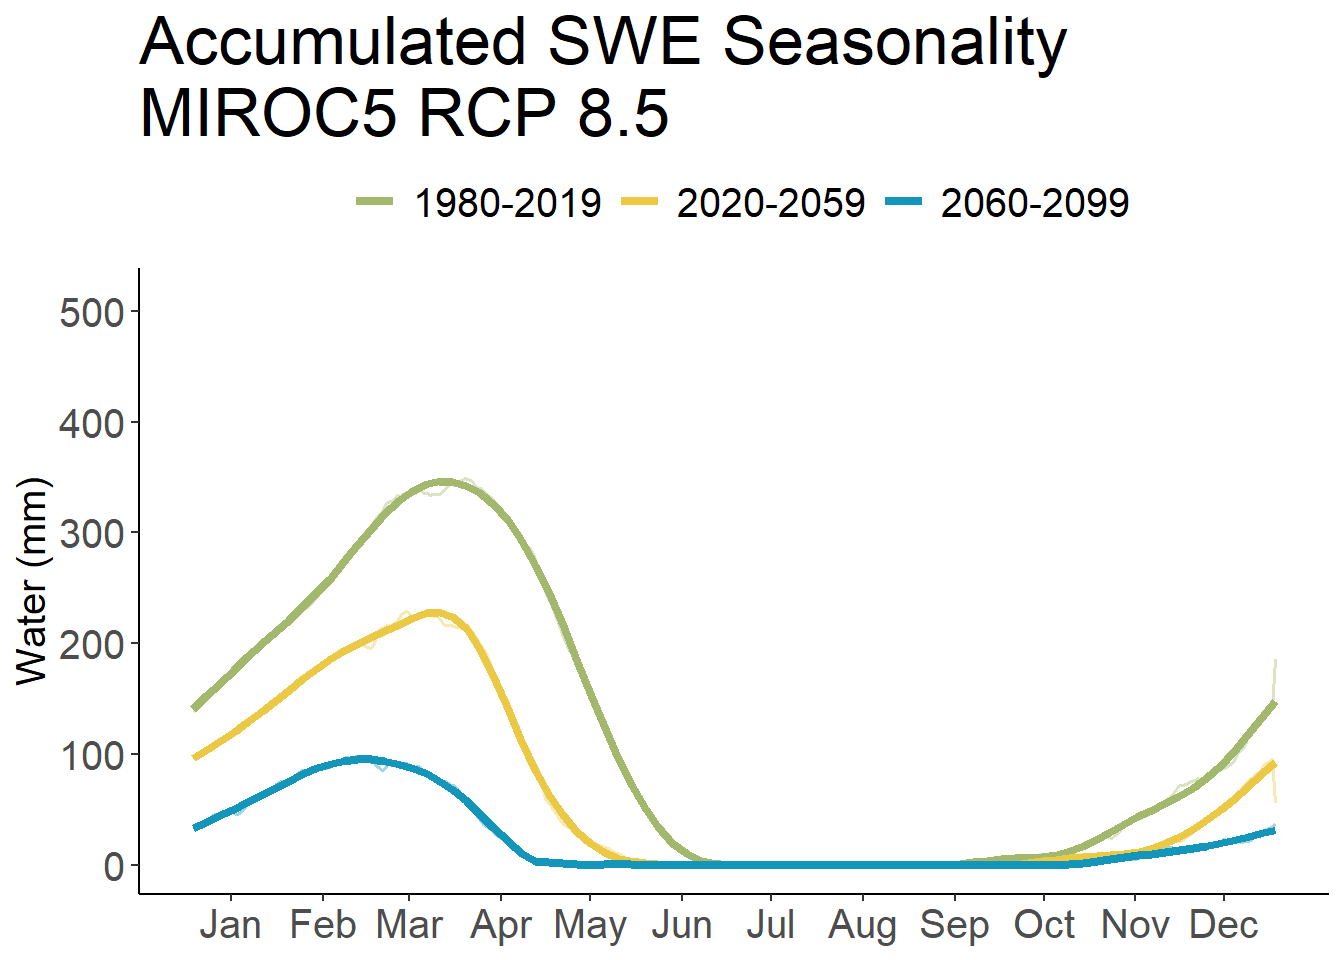
\includegraphics[width=0.5\linewidth]{water_balance_graphs_files/figure-latex/unnamed-chunk-23-2}
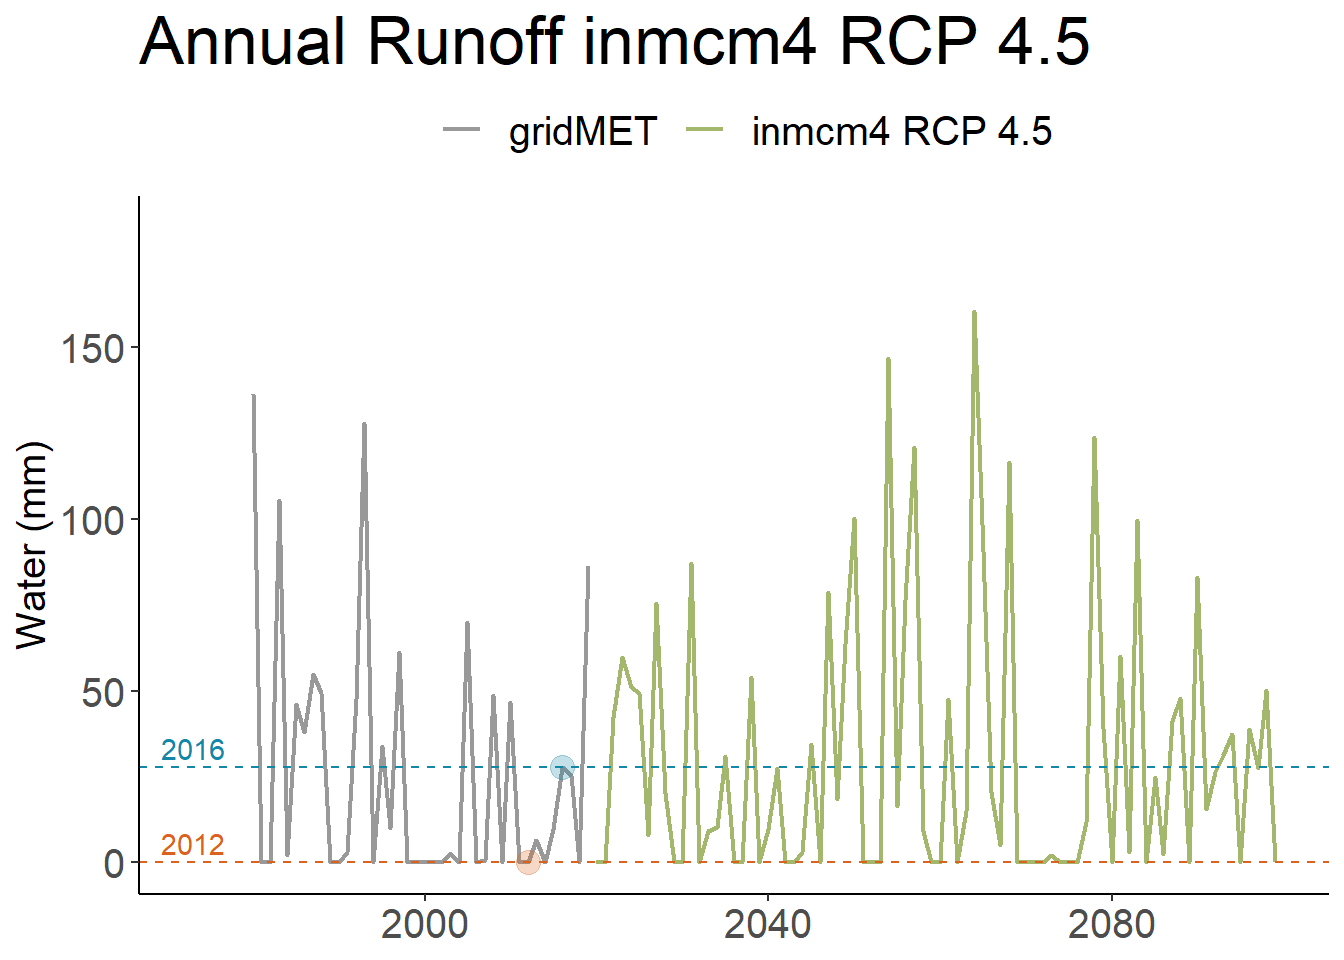
\includegraphics[width=0.5\linewidth]{water_balance_graphs_files/figure-latex/unnamed-chunk-23-3}
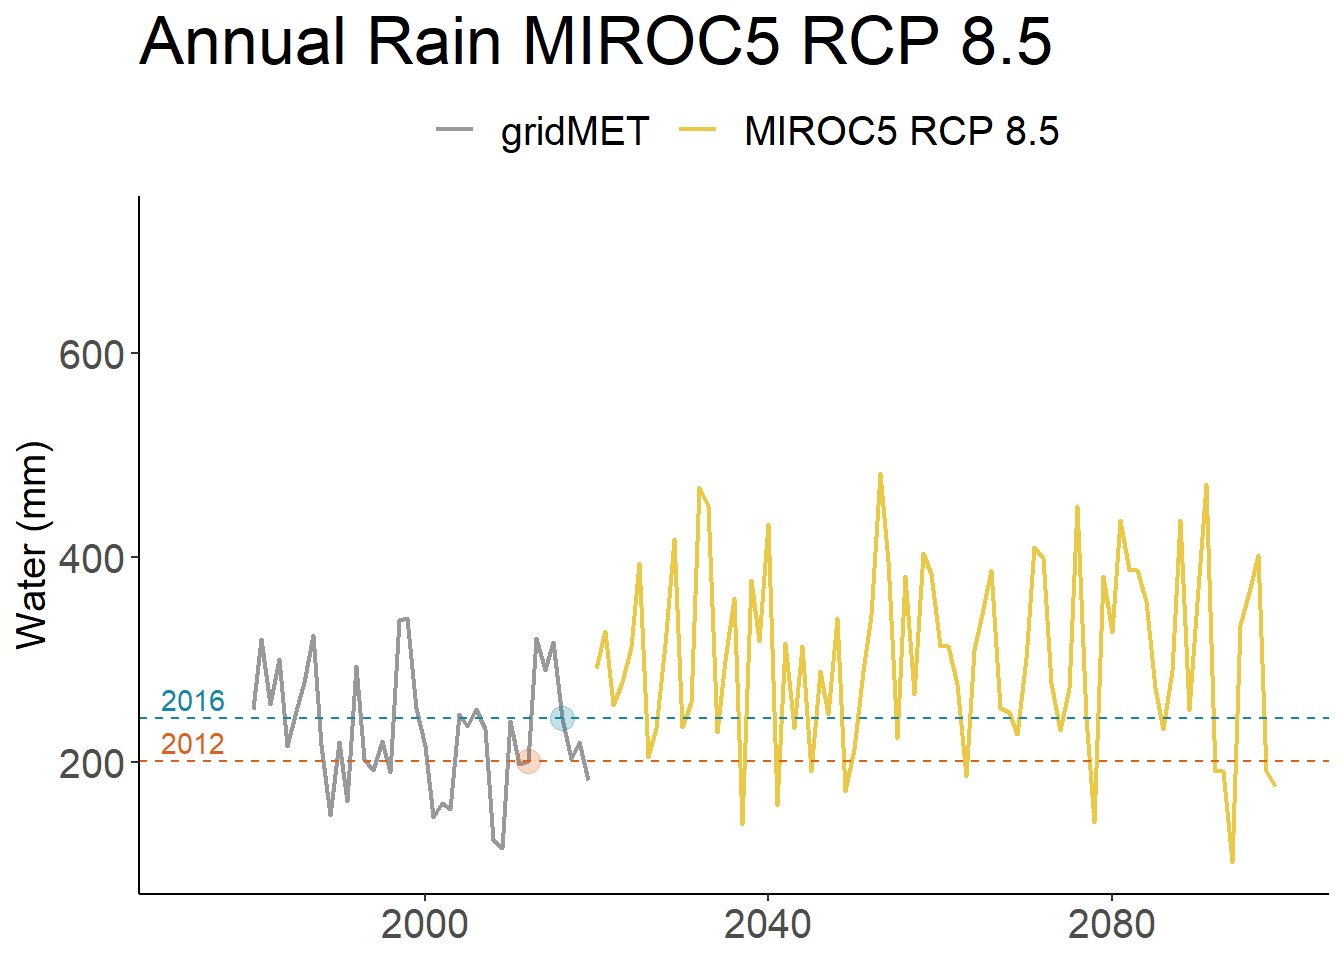
\includegraphics[width=0.5\linewidth]{water_balance_graphs_files/figure-latex/unnamed-chunk-23-4}
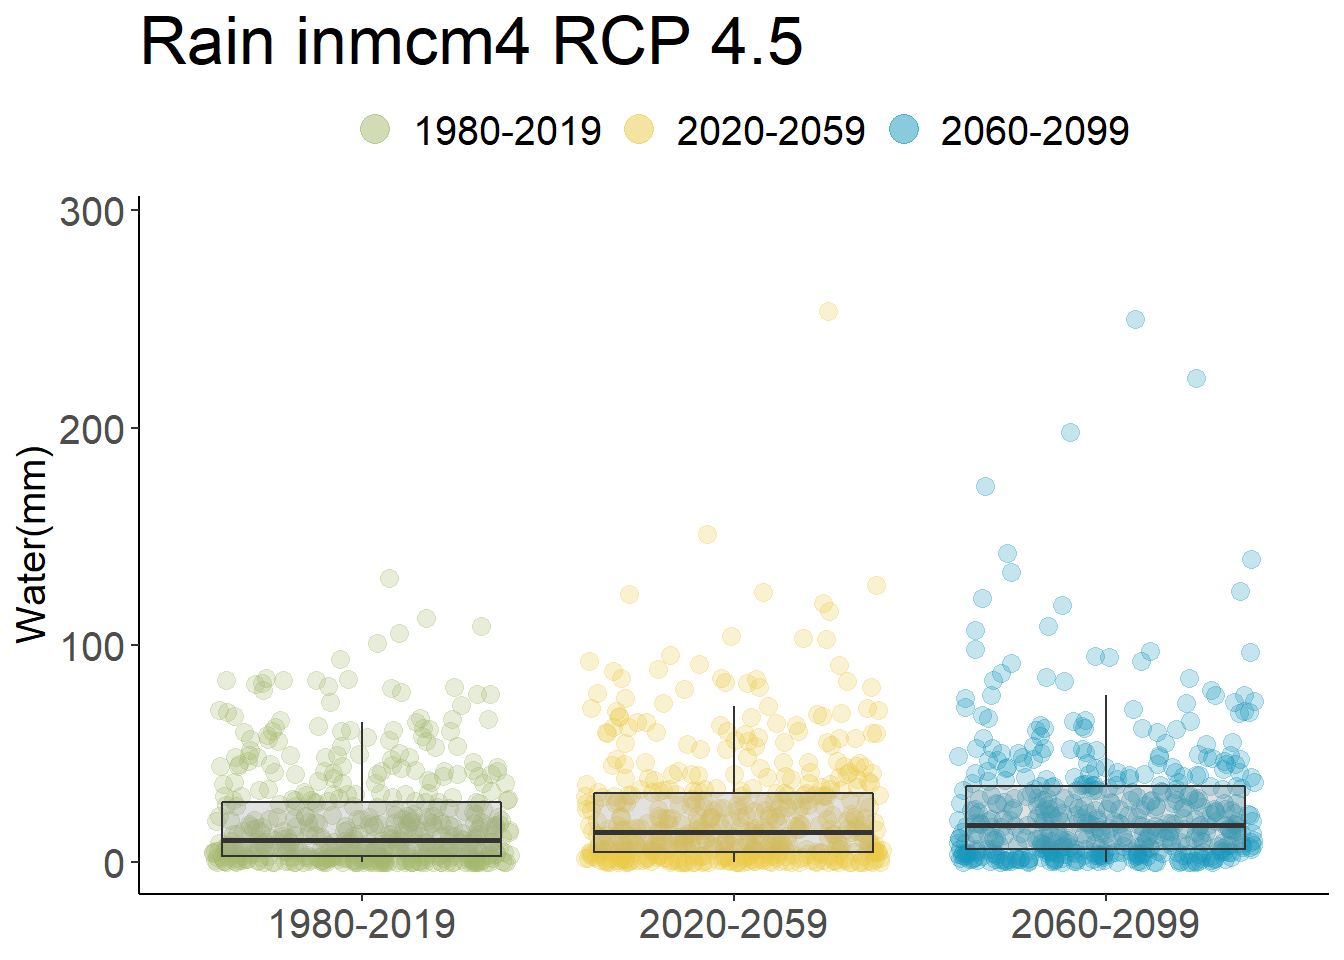
\includegraphics[width=0.5\linewidth]{water_balance_graphs_files/figure-latex/unnamed-chunk-23-5}
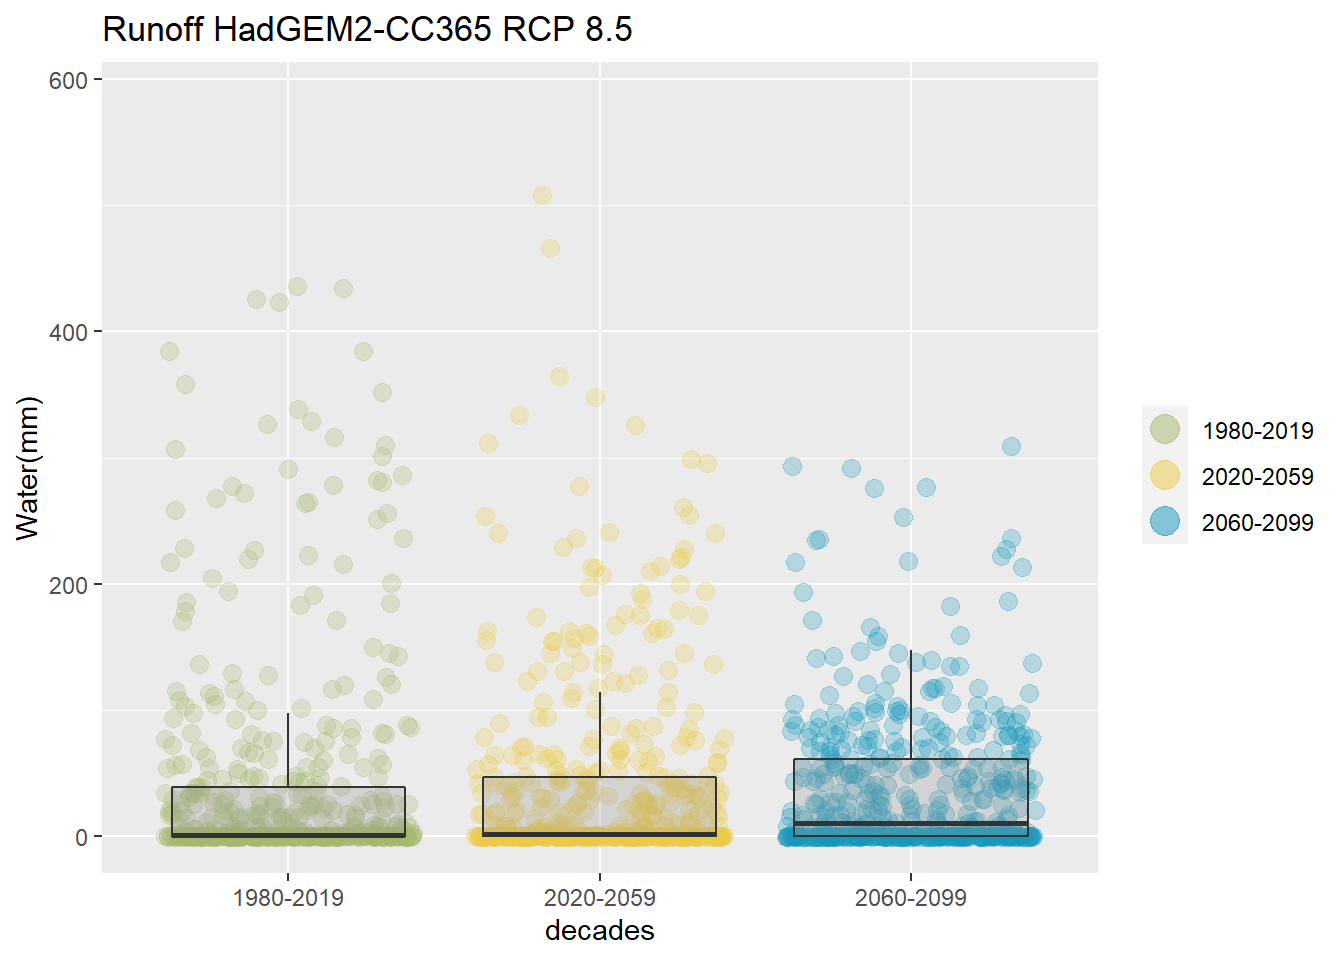
\includegraphics[width=0.5\linewidth]{water_balance_graphs_files/figure-latex/unnamed-chunk-23-6}

\hypertarget{accumulated-snow-water-equivalent-swe}{%
\subsection{Accumulated Snow Water Equivalent
(SWE)}\label{accumulated-snow-water-equivalent-swe}}

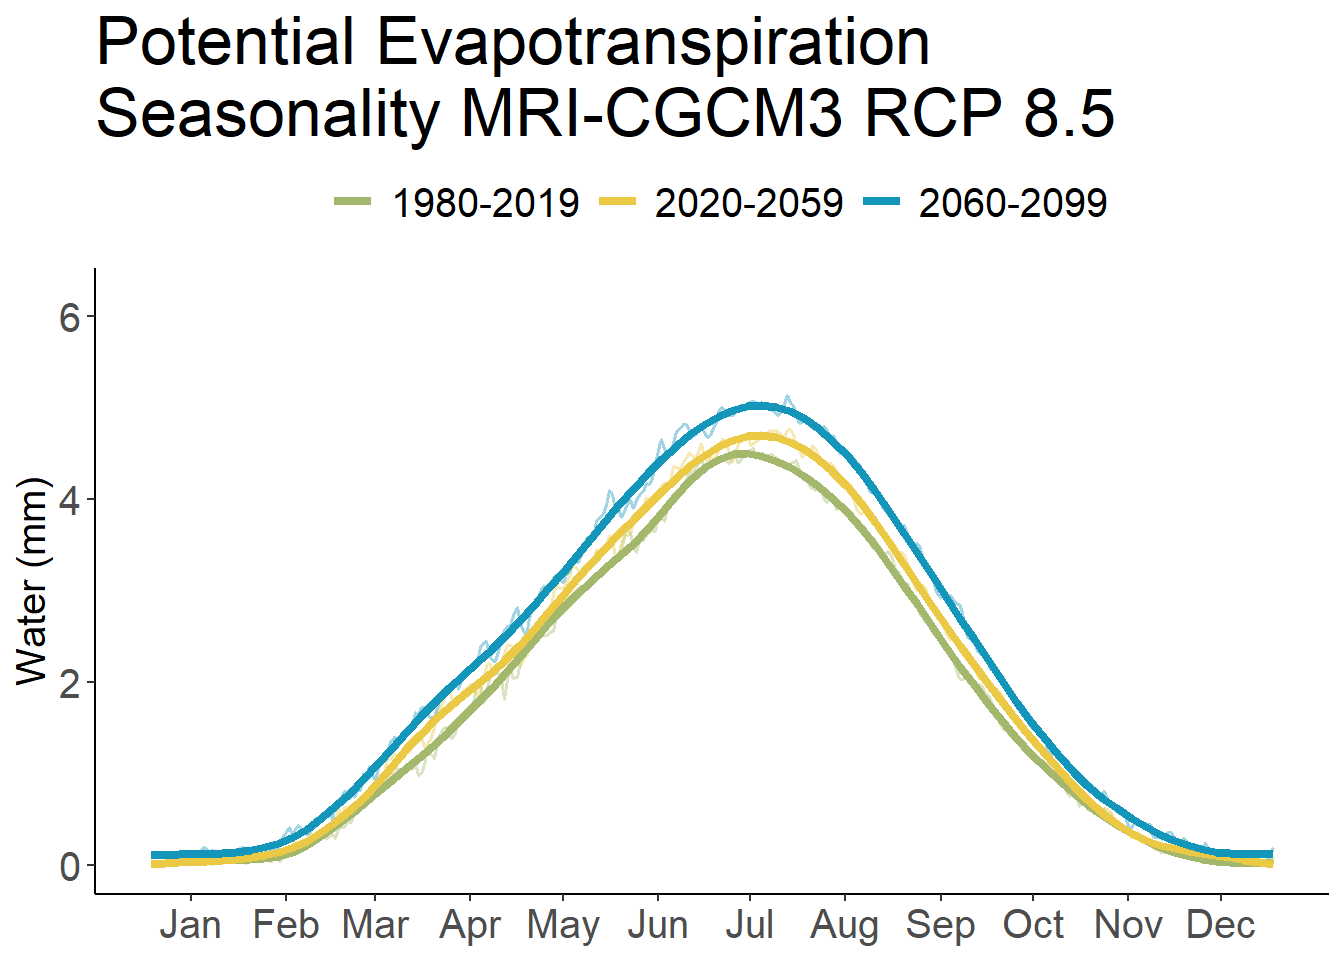
\includegraphics[width=0.5\linewidth]{water_balance_graphs_files/figure-latex/unnamed-chunk-24-1}
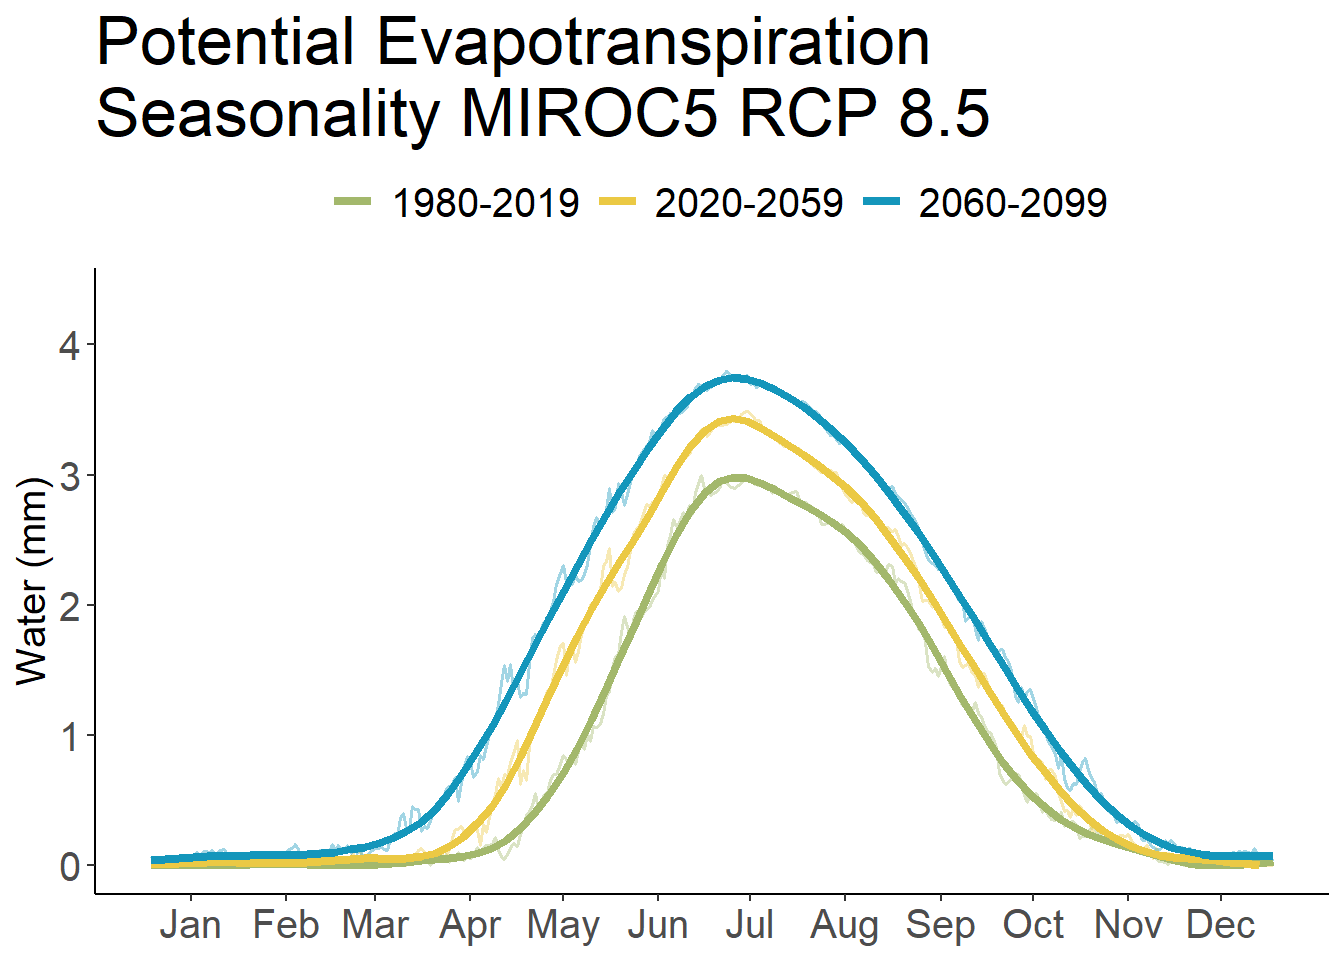
\includegraphics[width=0.5\linewidth]{water_balance_graphs_files/figure-latex/unnamed-chunk-24-2}
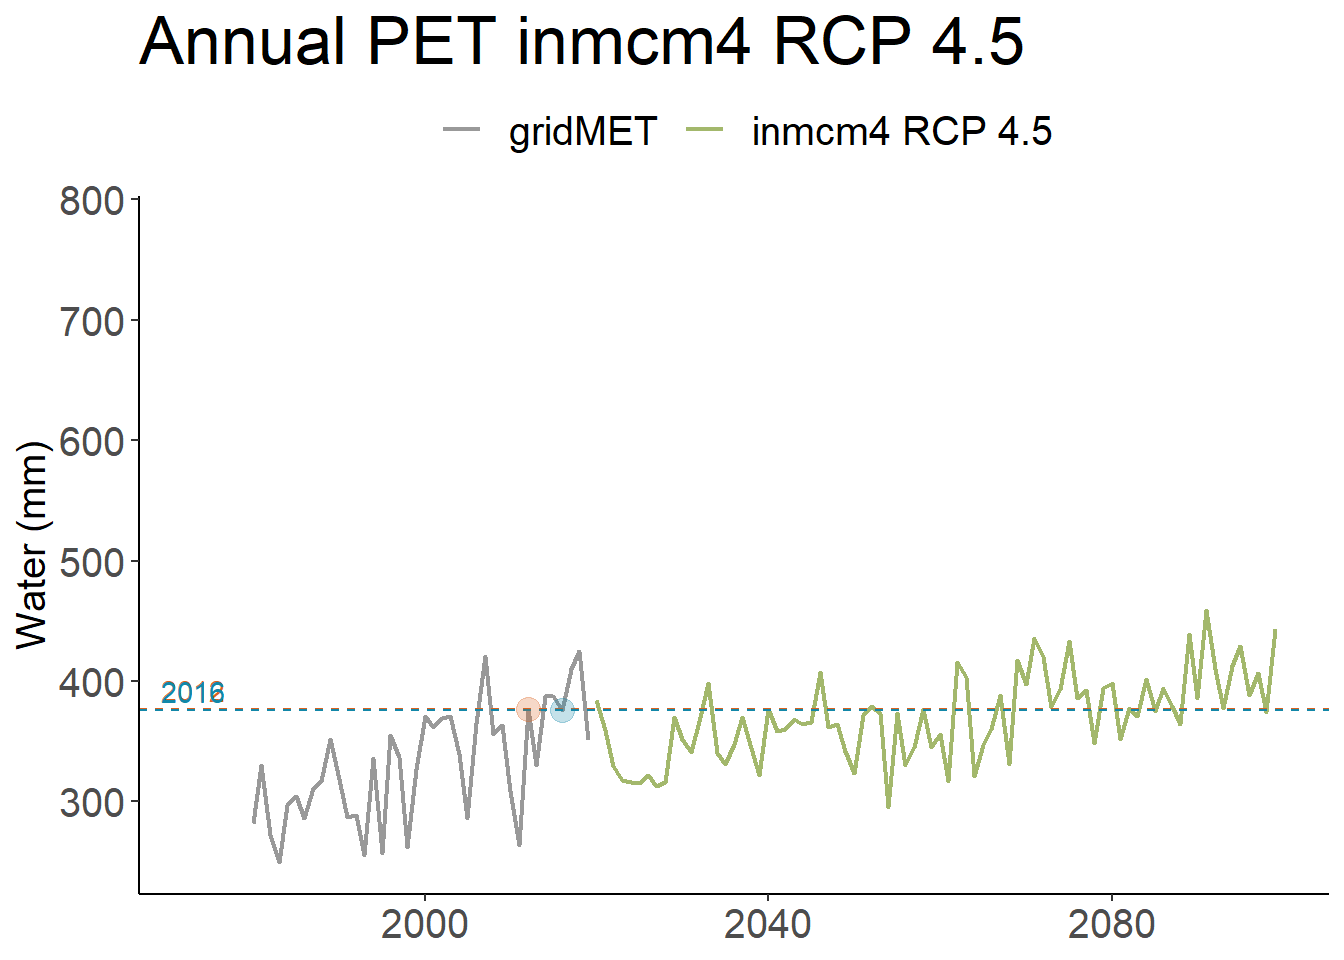
\includegraphics[width=0.5\linewidth]{water_balance_graphs_files/figure-latex/unnamed-chunk-24-3}
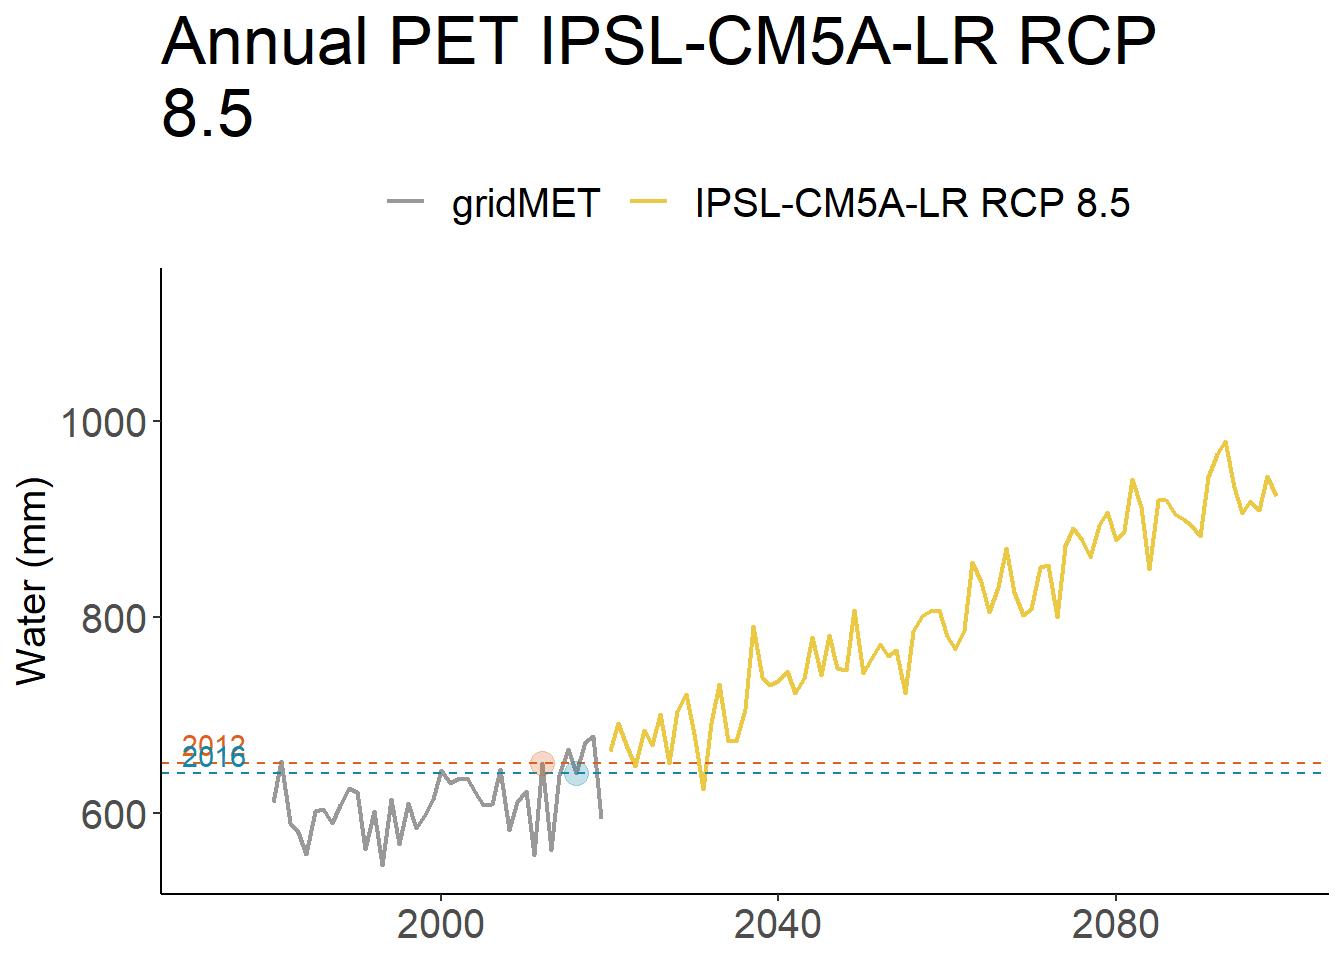
\includegraphics[width=0.5\linewidth]{water_balance_graphs_files/figure-latex/unnamed-chunk-24-4}
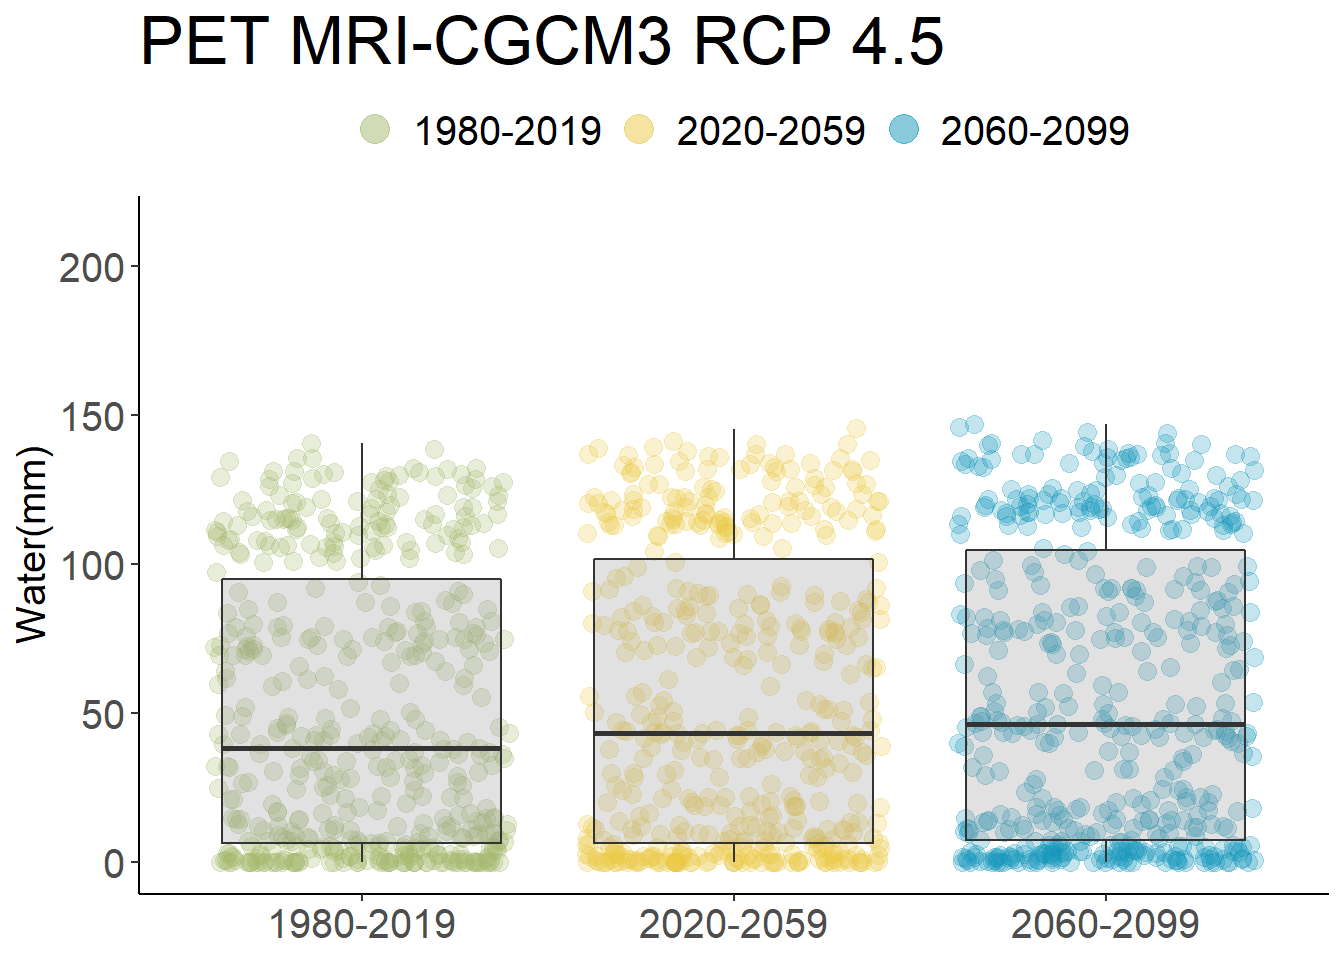
\includegraphics[width=0.5\linewidth]{water_balance_graphs_files/figure-latex/unnamed-chunk-24-5}
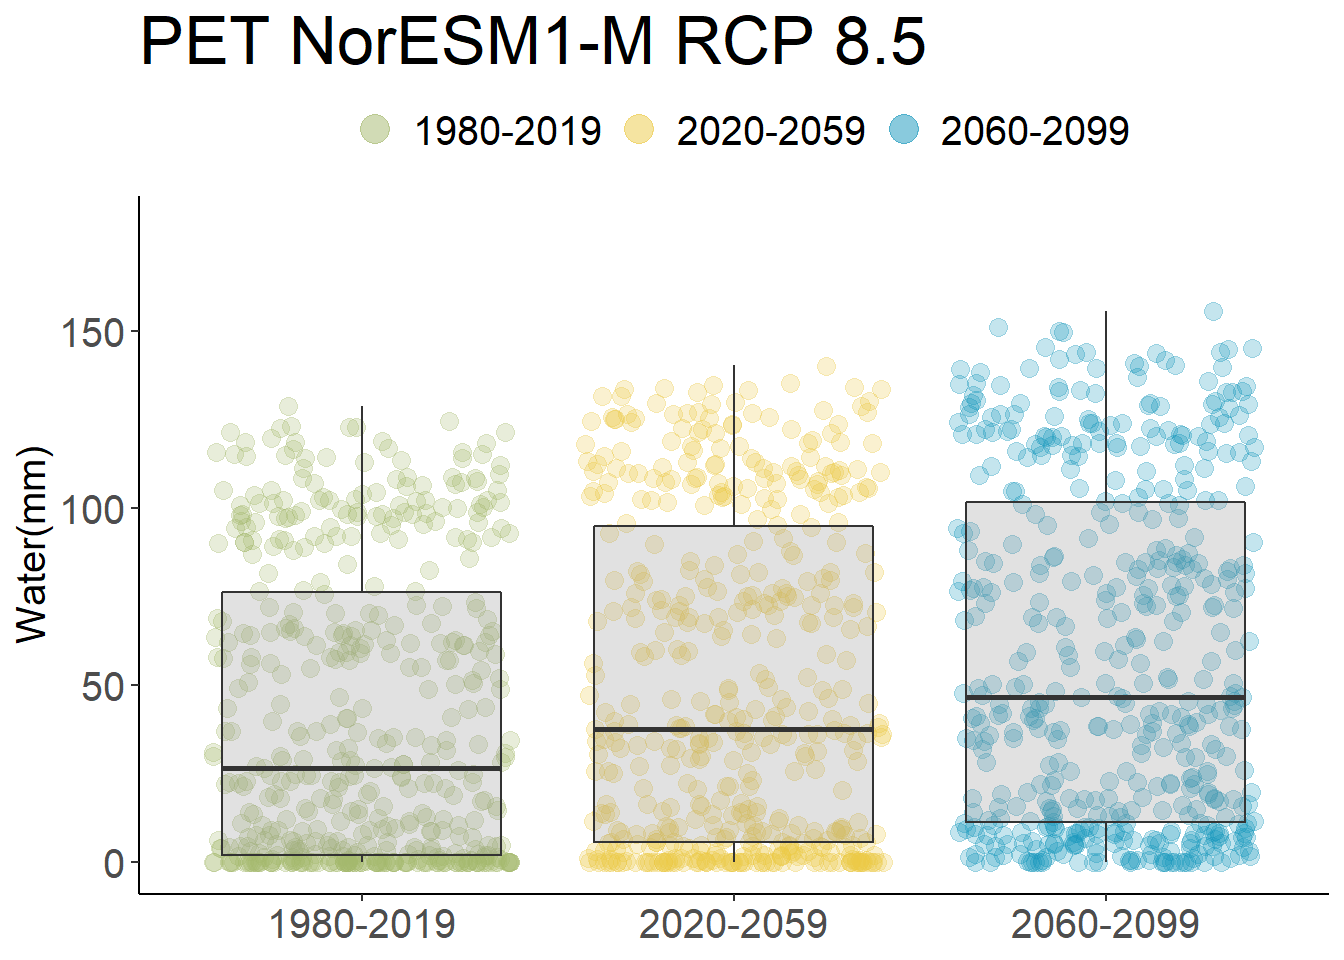
\includegraphics[width=0.5\linewidth]{water_balance_graphs_files/figure-latex/unnamed-chunk-24-6}

\hypertarget{potential-evapotranspiration-pet}{%
\subsection{Potential Evapotranspiration
(PET)}\label{potential-evapotranspiration-pet}}

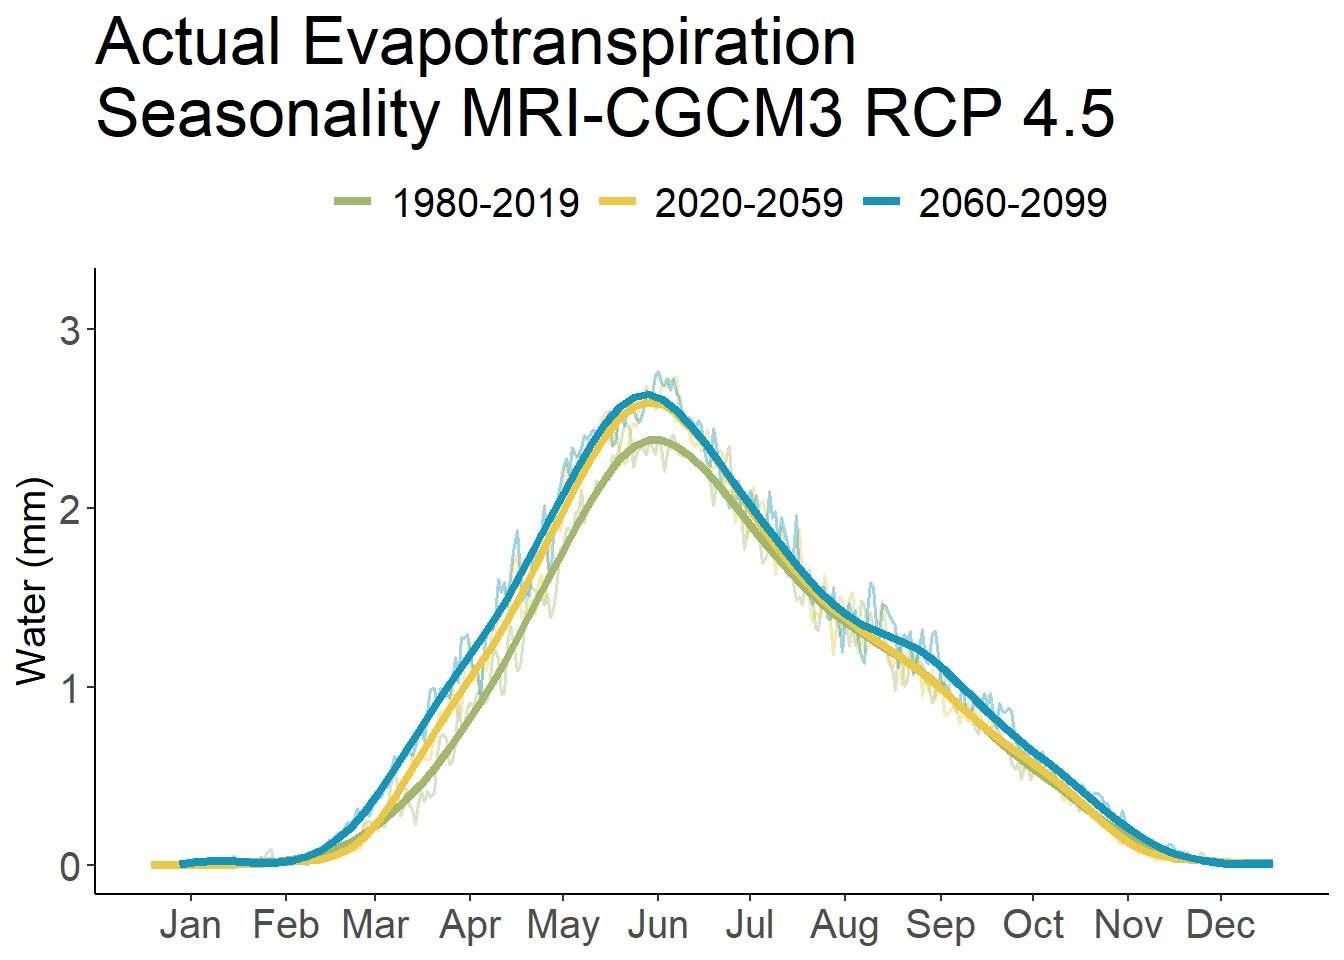
\includegraphics[width=0.5\linewidth]{water_balance_graphs_files/figure-latex/unnamed-chunk-25-1}
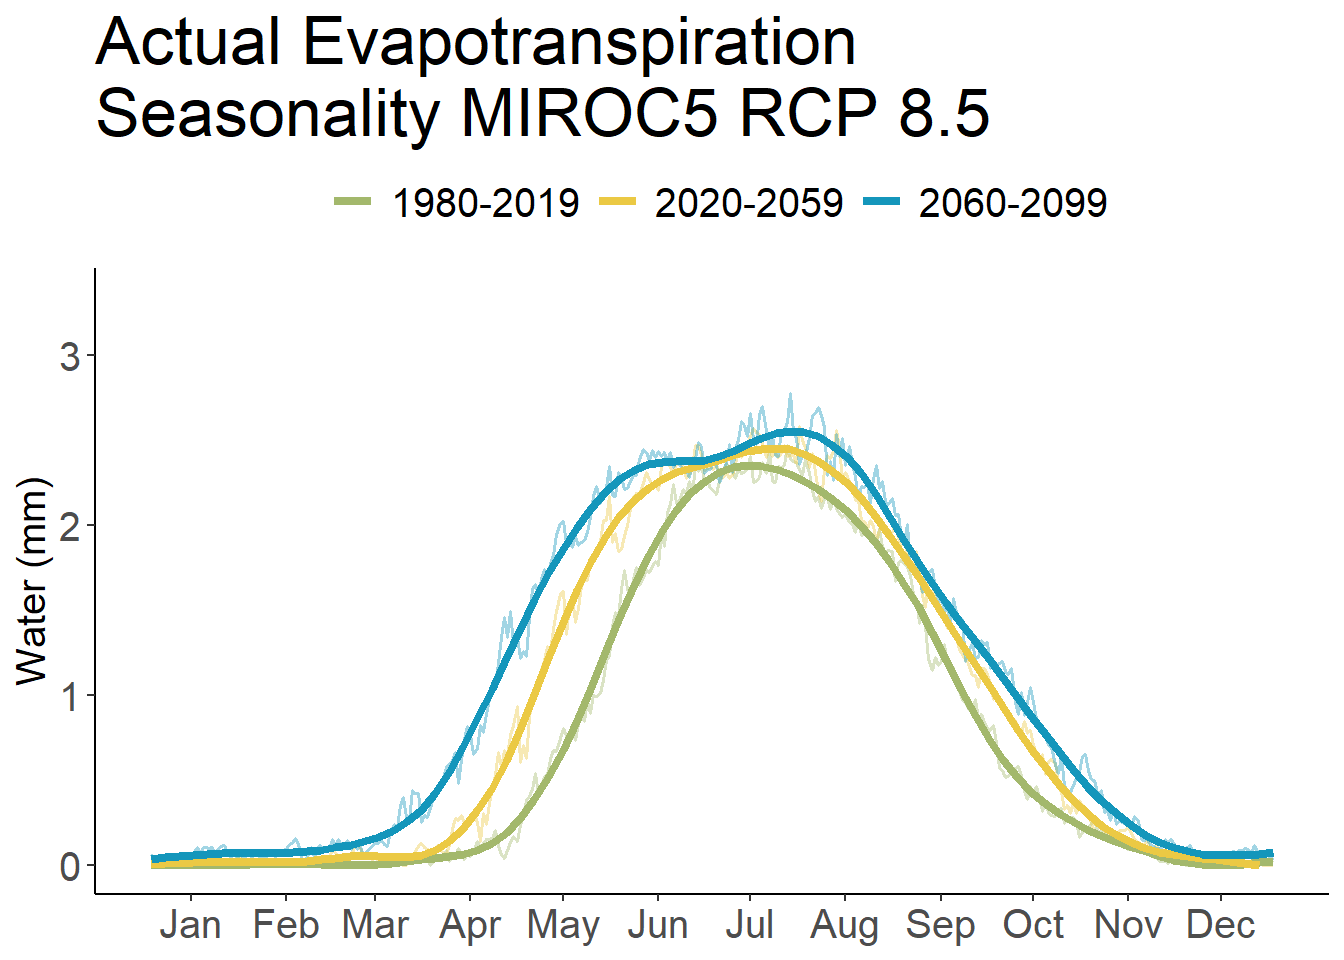
\includegraphics[width=0.5\linewidth]{water_balance_graphs_files/figure-latex/unnamed-chunk-25-2}
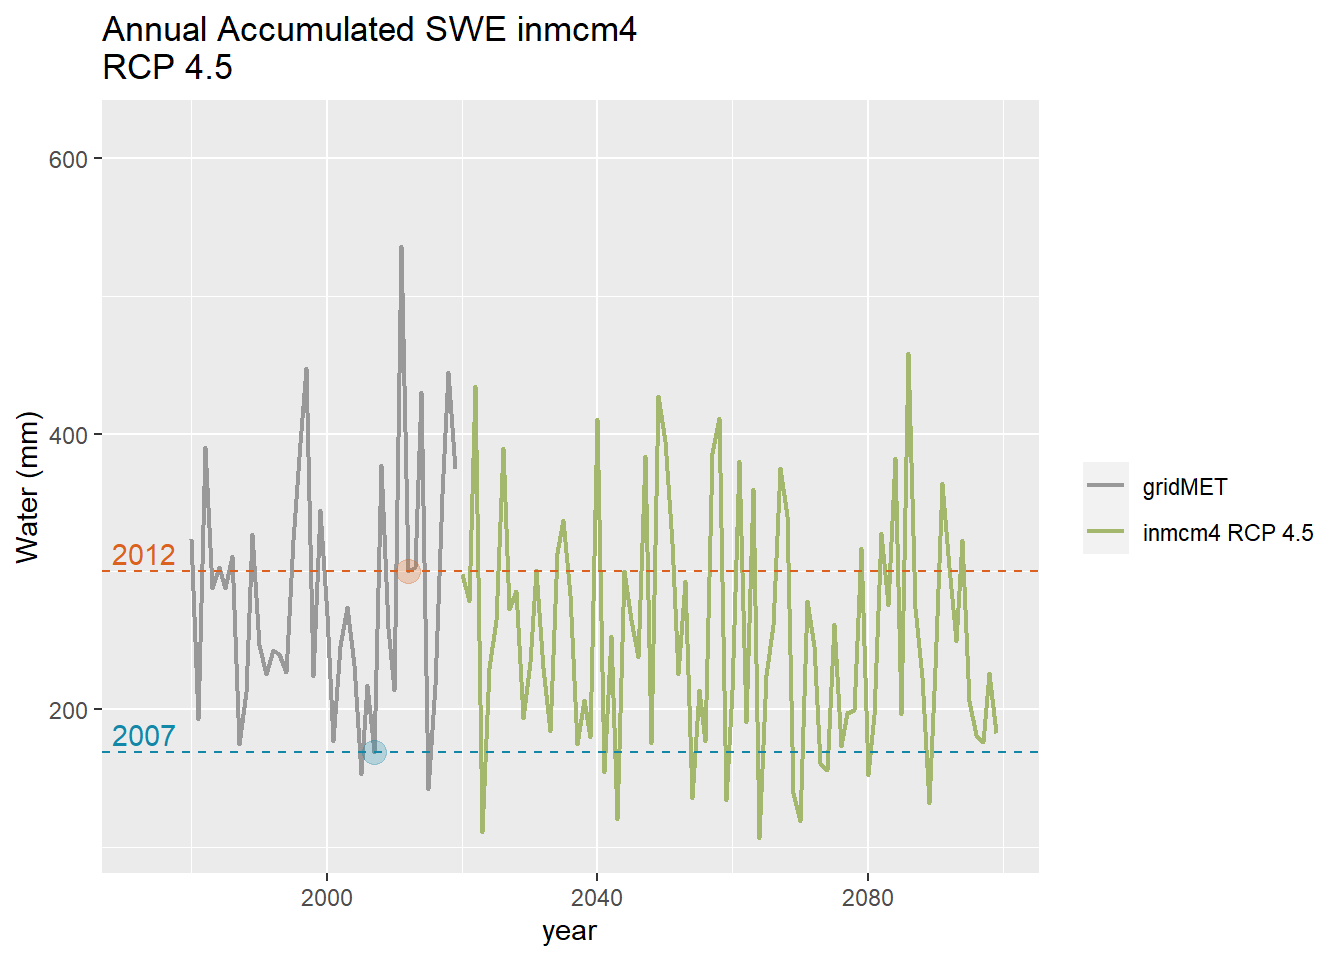
\includegraphics[width=0.5\linewidth]{water_balance_graphs_files/figure-latex/unnamed-chunk-25-3}
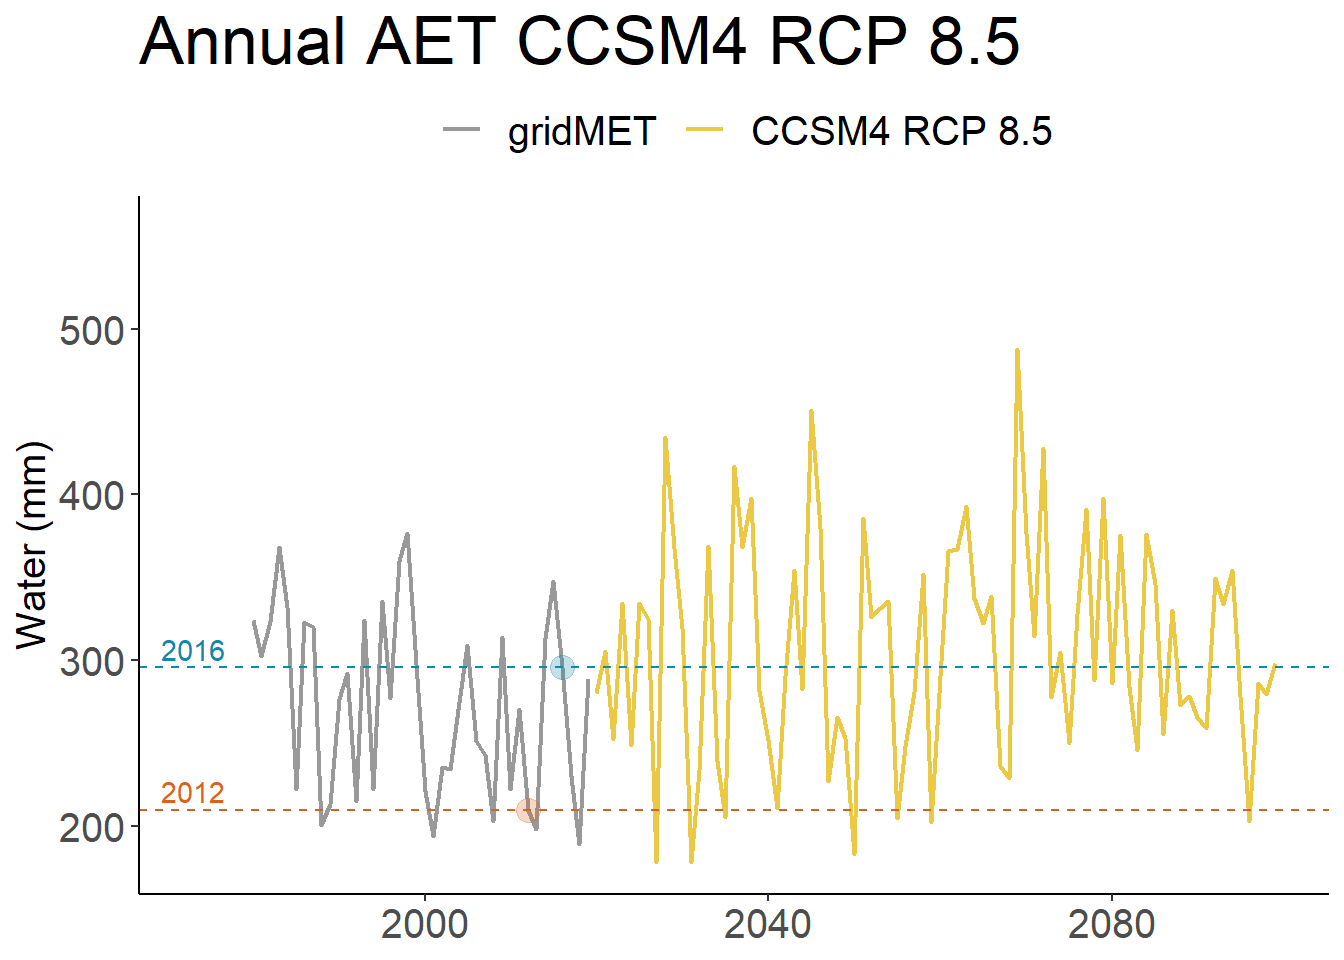
\includegraphics[width=0.5\linewidth]{water_balance_graphs_files/figure-latex/unnamed-chunk-25-4}

\hypertarget{actual-evapotranspiration-aet}{%
\subsection{Actual Evapotranspiration
(AET)}\label{actual-evapotranspiration-aet}}

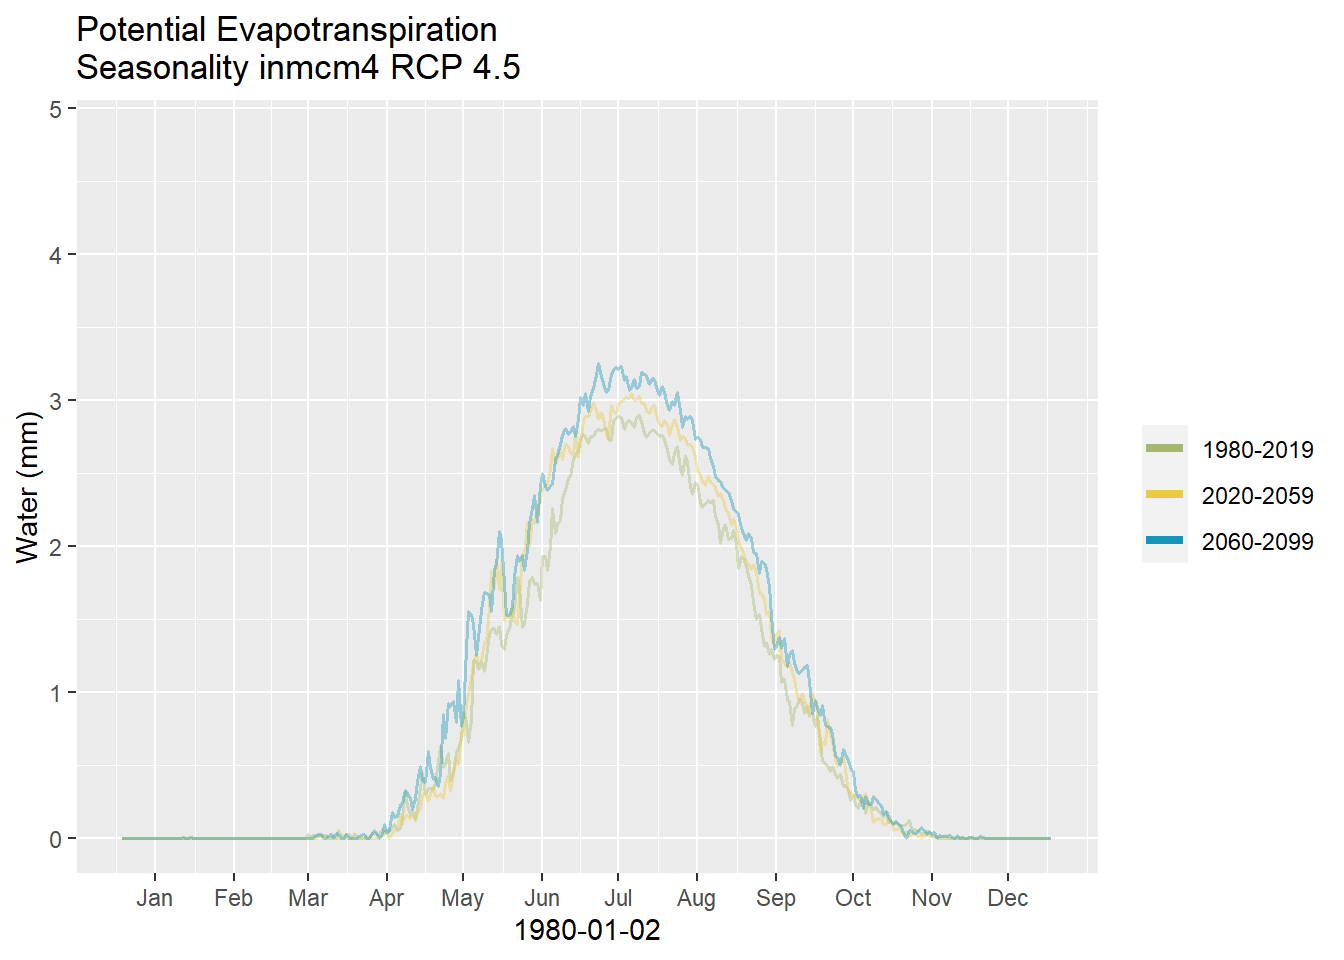
\includegraphics[width=0.5\linewidth]{water_balance_graphs_files/figure-latex/unnamed-chunk-26-1}
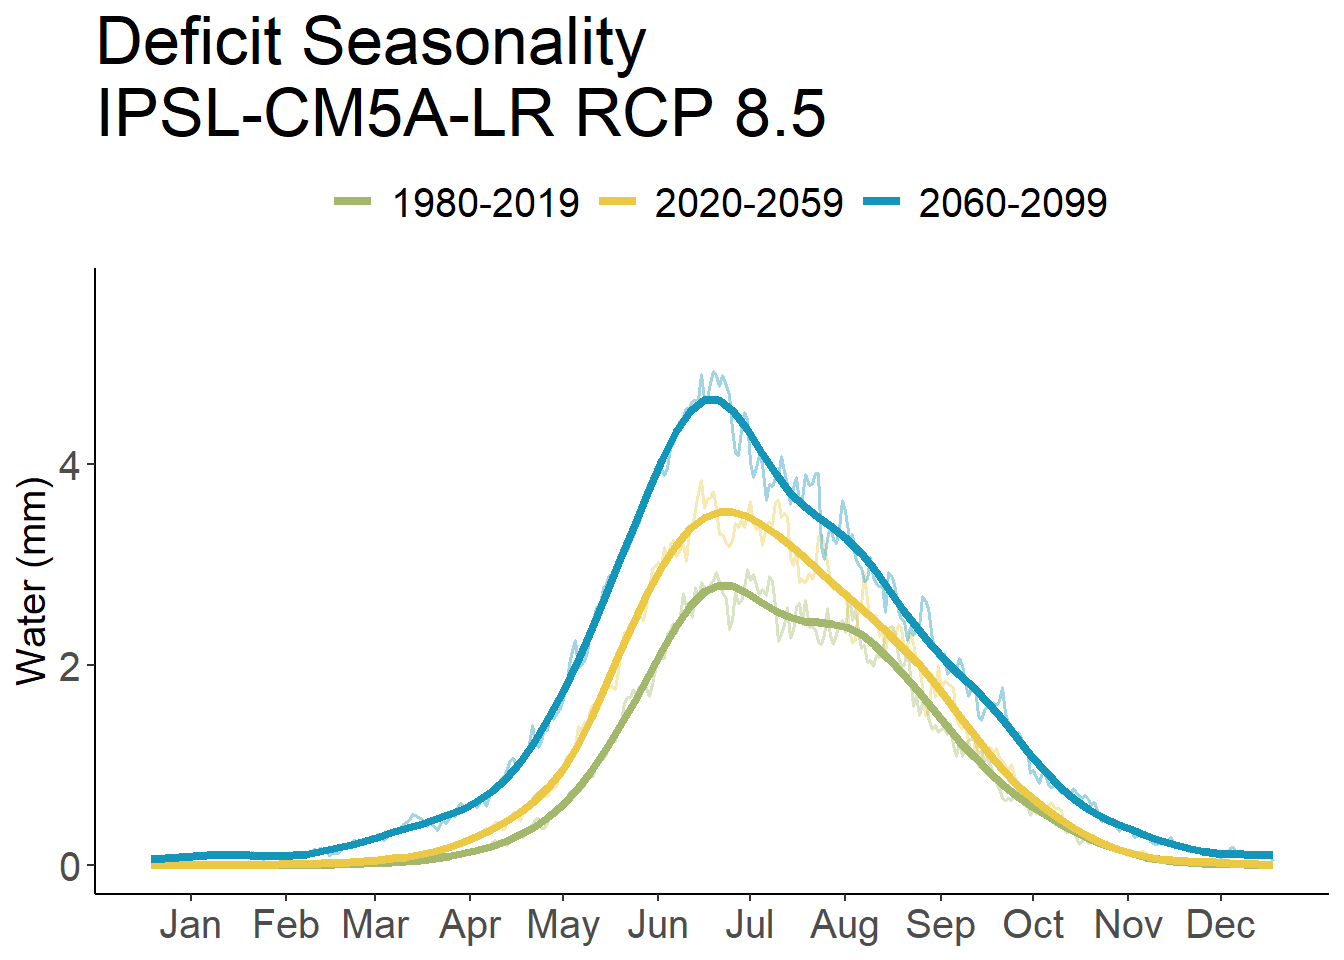
\includegraphics[width=0.5\linewidth]{water_balance_graphs_files/figure-latex/unnamed-chunk-26-2}
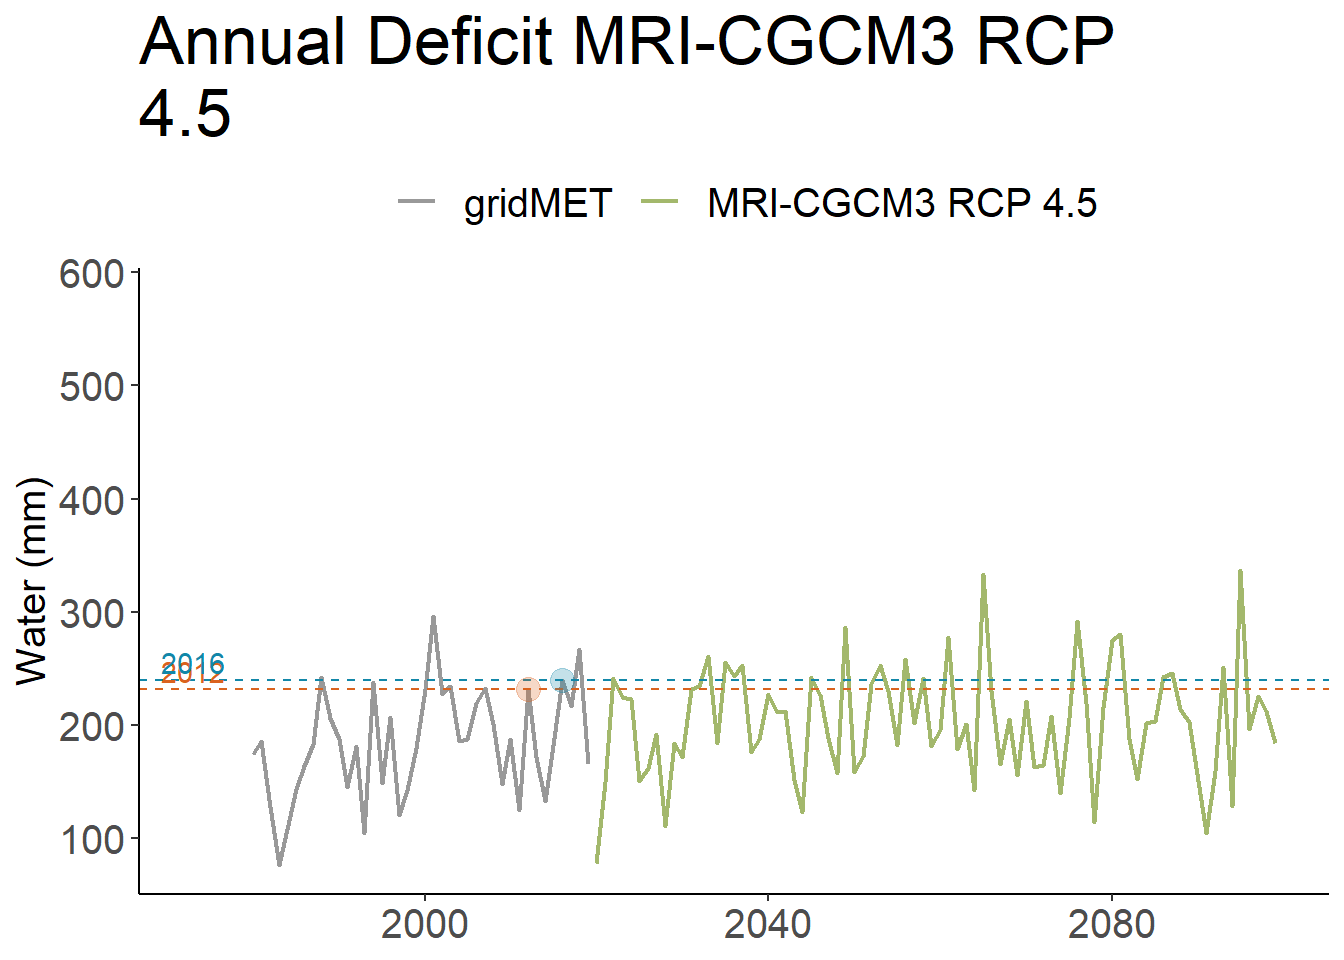
\includegraphics[width=0.5\linewidth]{water_balance_graphs_files/figure-latex/unnamed-chunk-26-3}
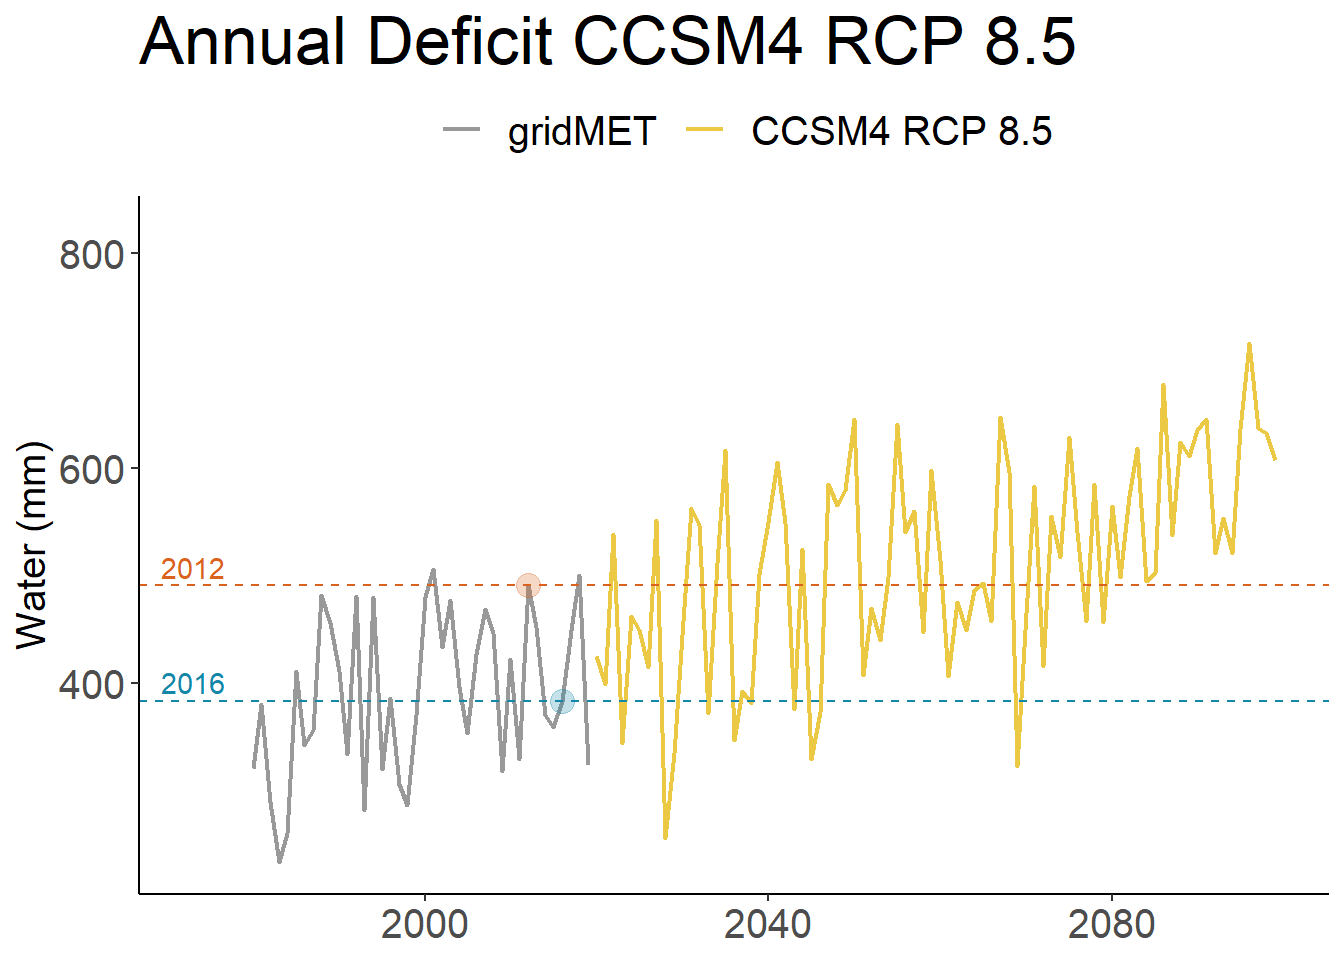
\includegraphics[width=0.5\linewidth]{water_balance_graphs_files/figure-latex/unnamed-chunk-26-4}
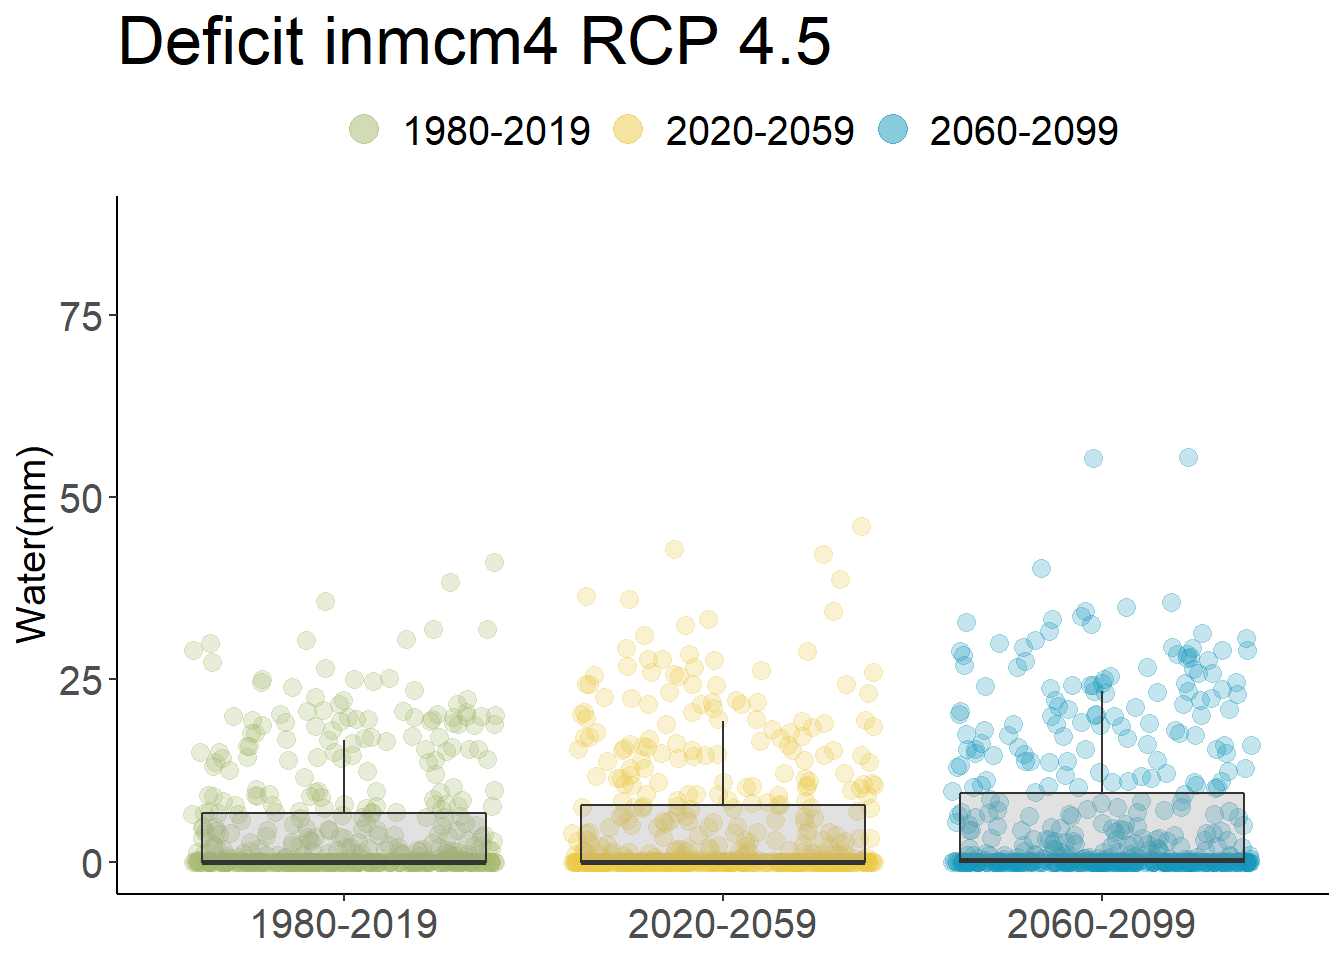
\includegraphics[width=0.5\linewidth]{water_balance_graphs_files/figure-latex/unnamed-chunk-26-5}
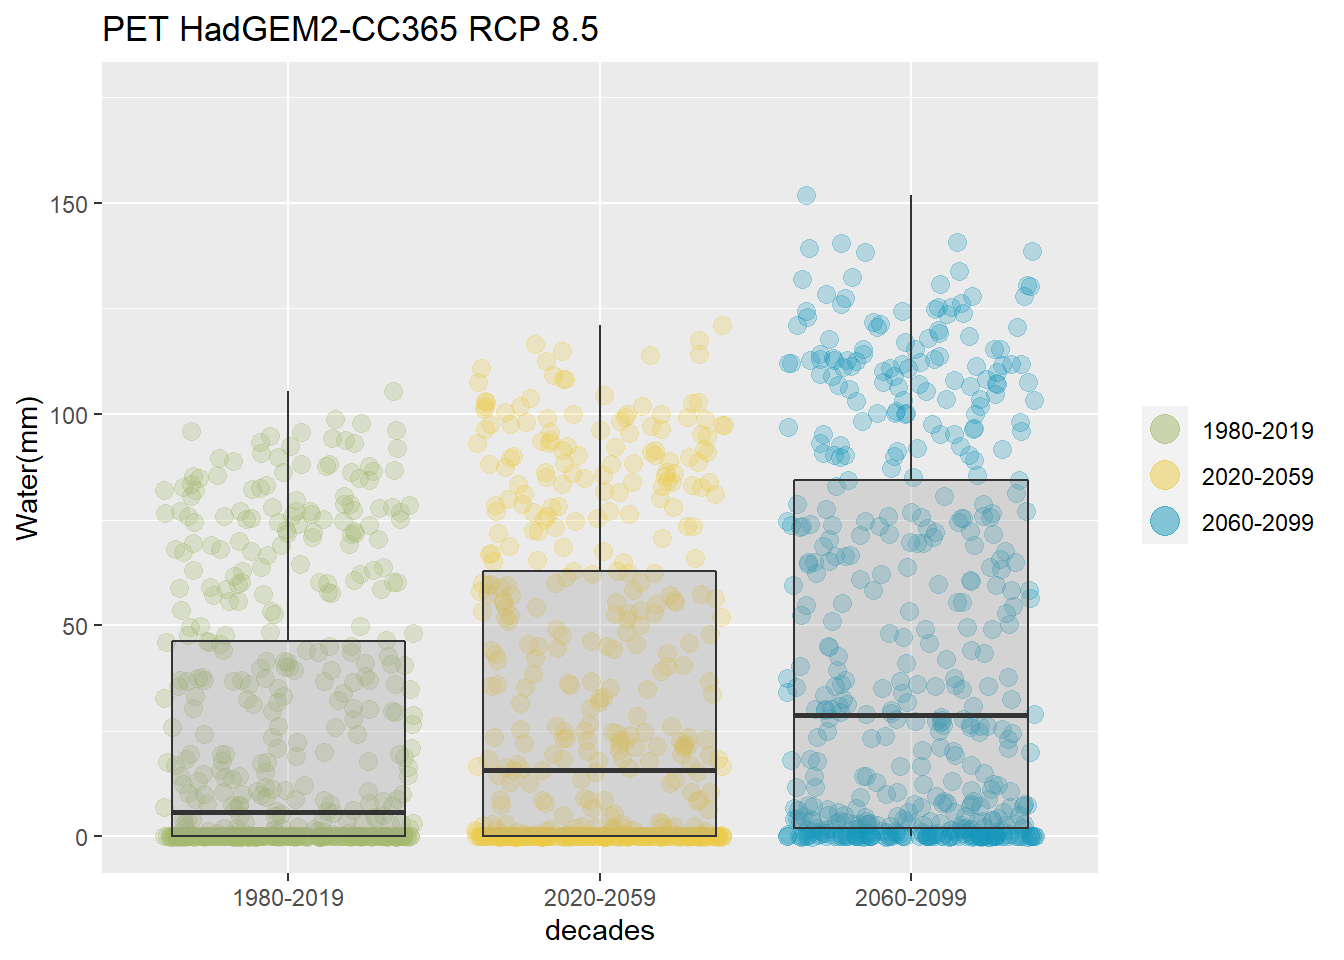
\includegraphics[width=0.5\linewidth]{water_balance_graphs_files/figure-latex/unnamed-chunk-26-6}

\hypertarget{deficit}{%
\subsection{Deficit}\label{deficit}}

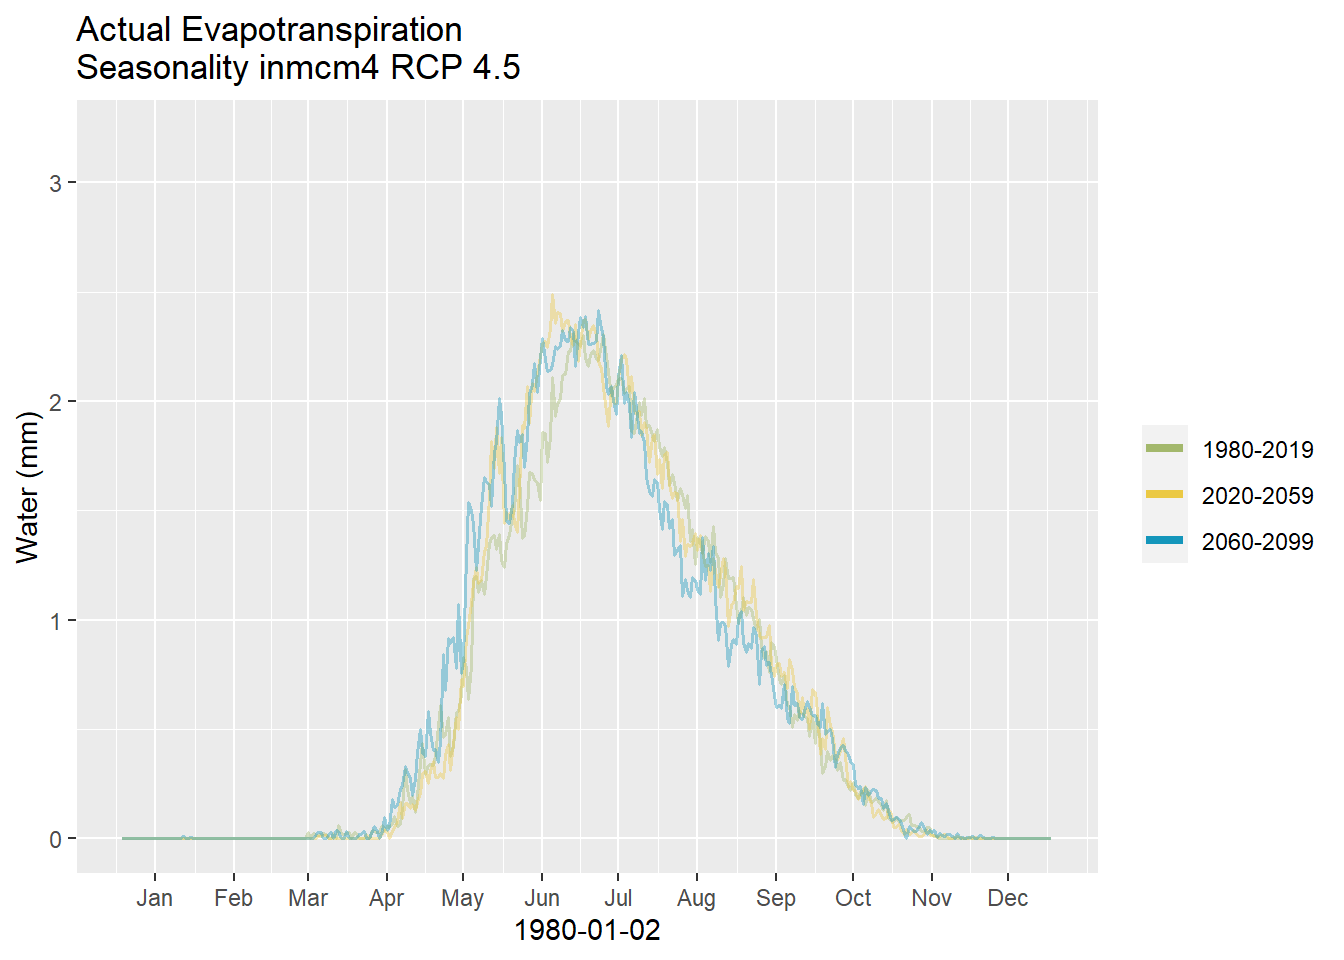
\includegraphics[width=0.5\linewidth]{water_balance_graphs_files/figure-latex/unnamed-chunk-27-1}
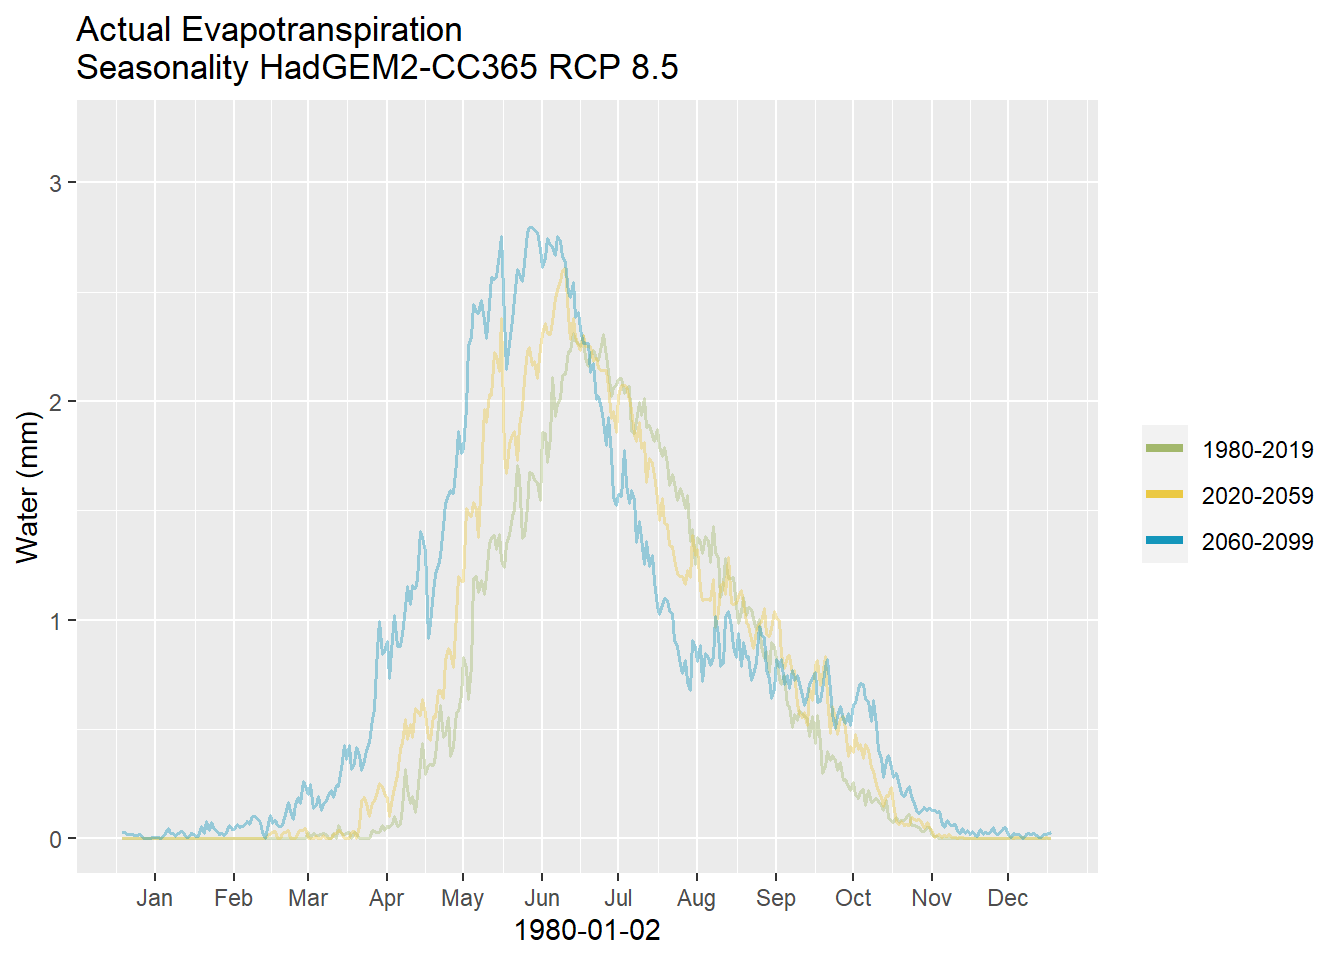
\includegraphics[width=0.5\linewidth]{water_balance_graphs_files/figure-latex/unnamed-chunk-27-2}
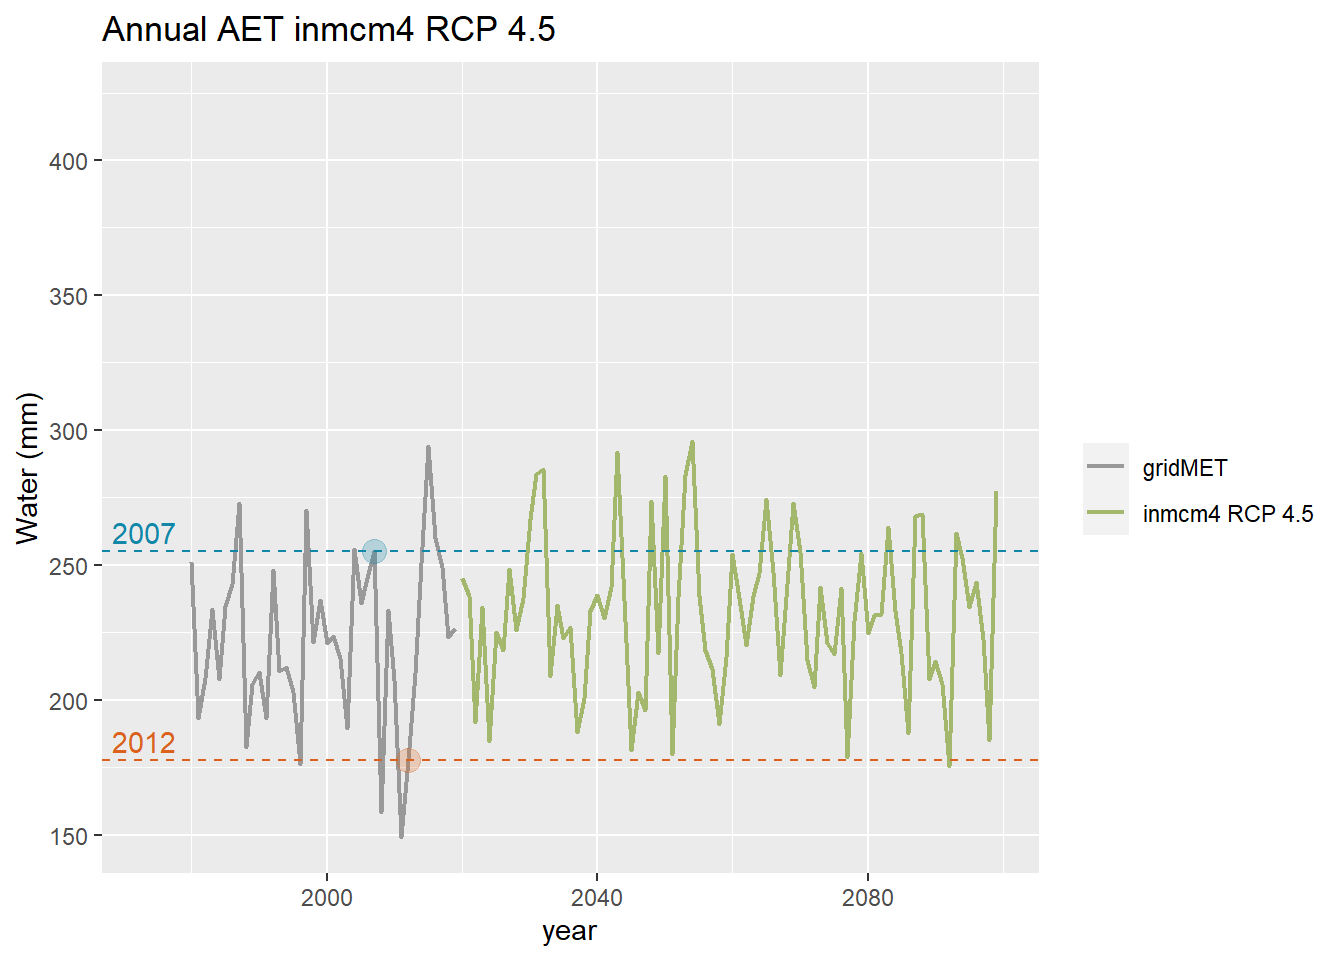
\includegraphics[width=0.5\linewidth]{water_balance_graphs_files/figure-latex/unnamed-chunk-27-3}
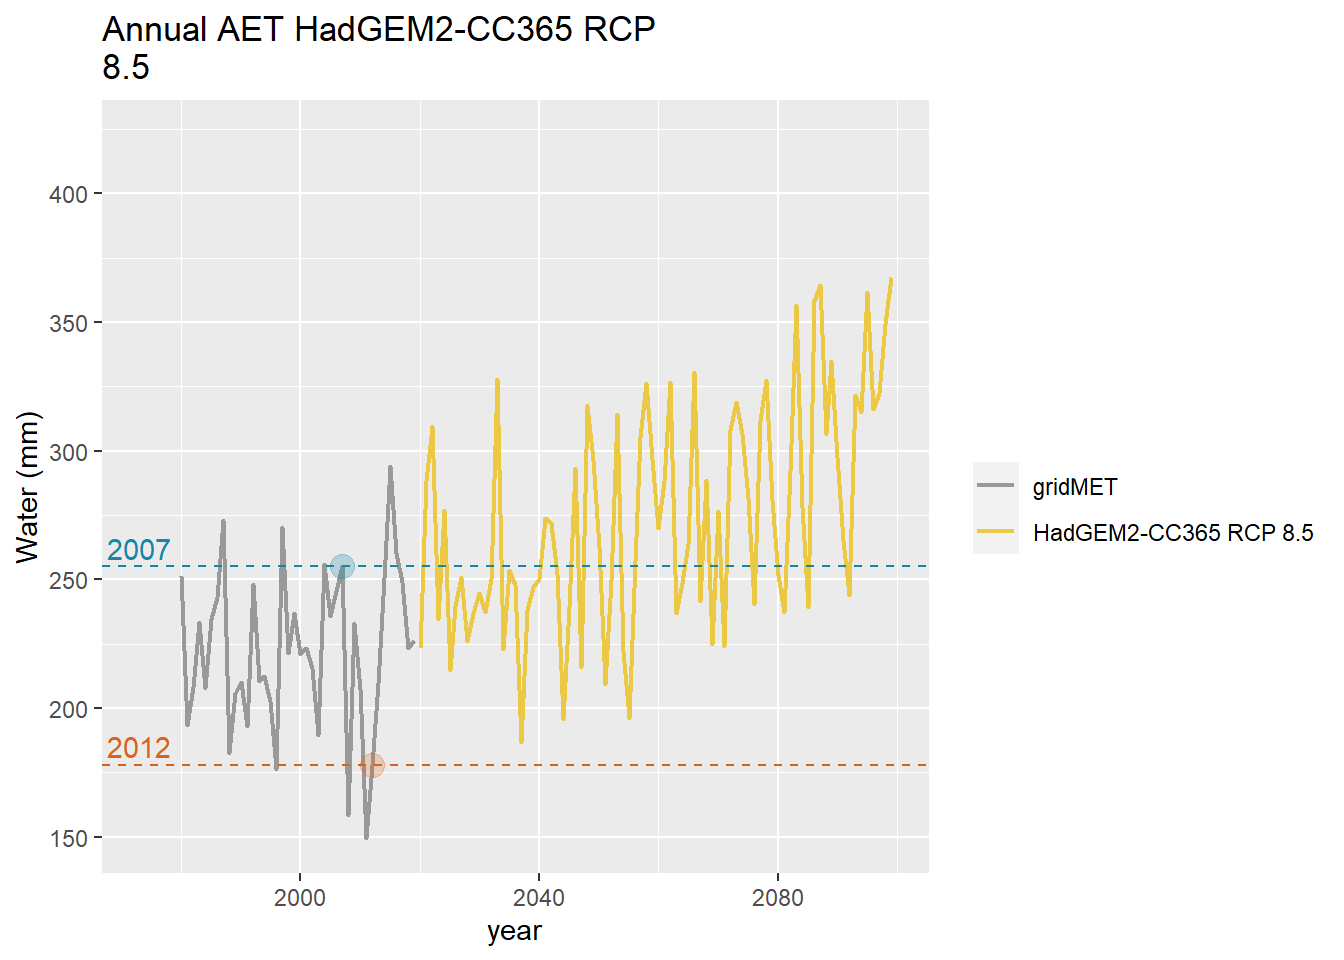
\includegraphics[width=0.5\linewidth]{water_balance_graphs_files/figure-latex/unnamed-chunk-27-4}
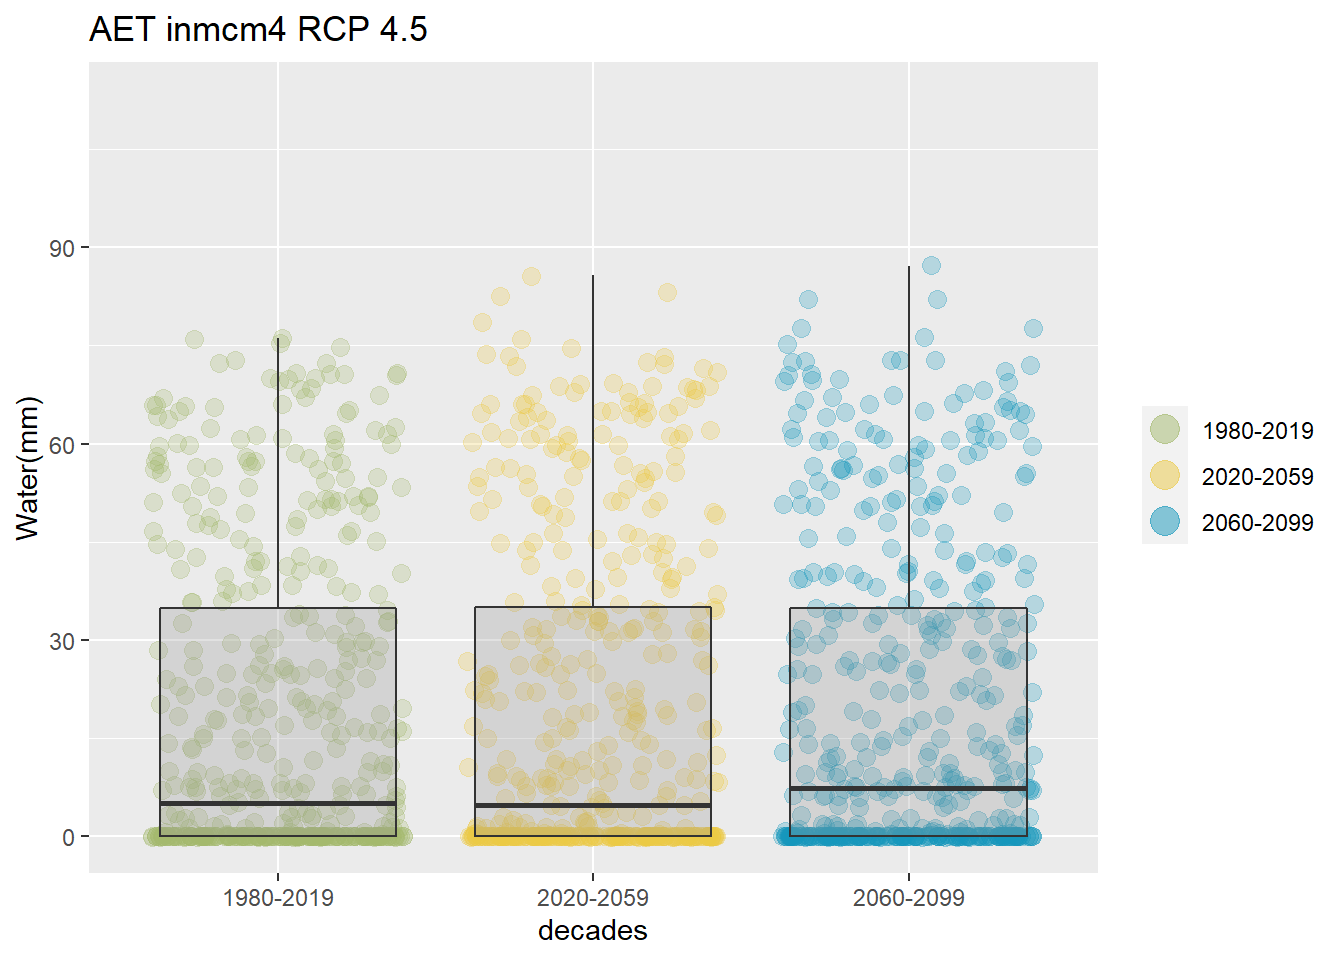
\includegraphics[width=0.5\linewidth]{water_balance_graphs_files/figure-latex/unnamed-chunk-27-5}
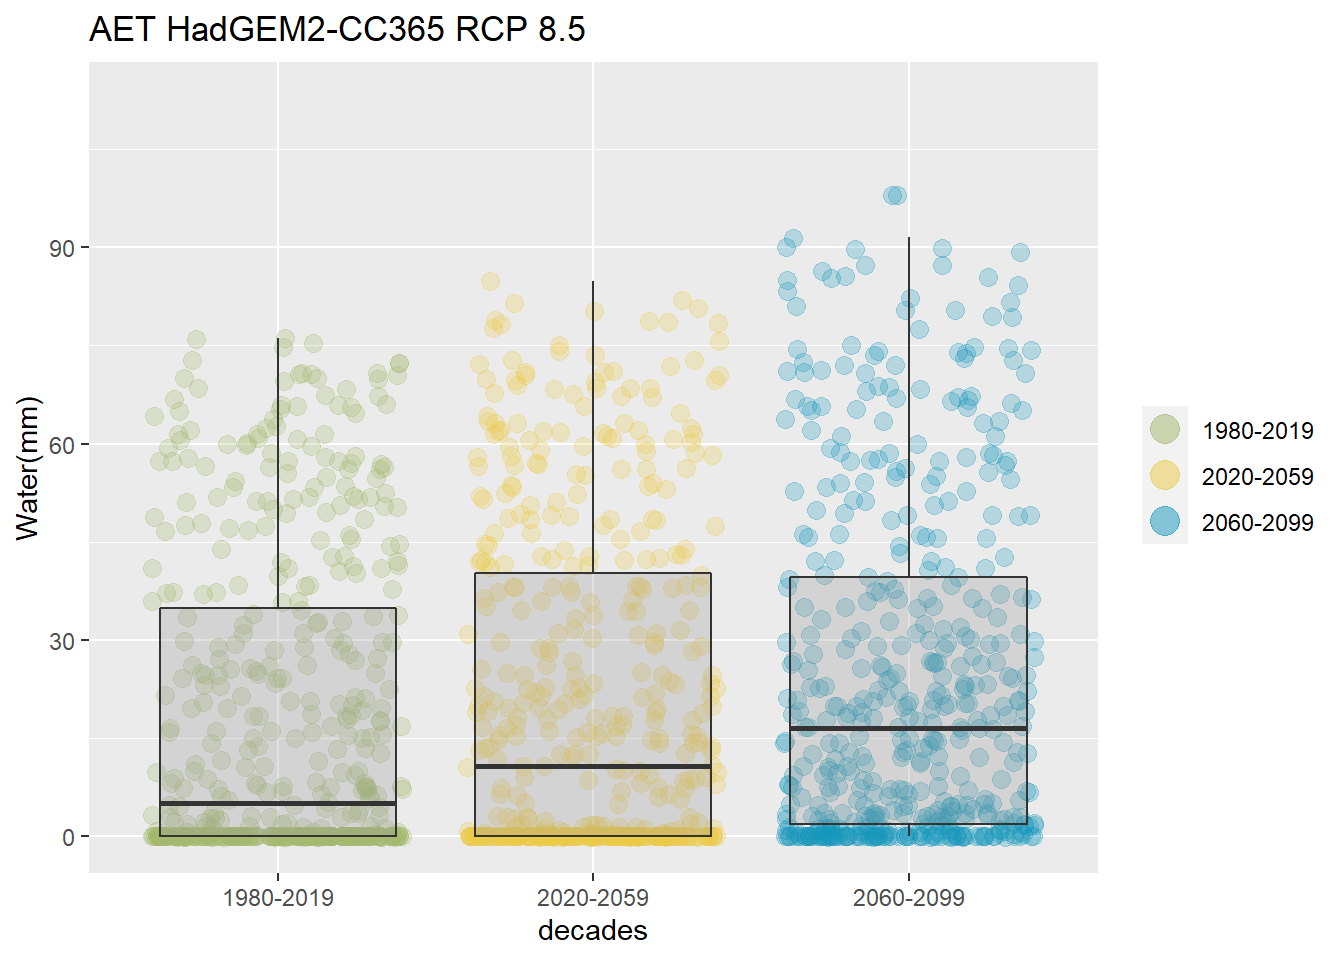
\includegraphics[width=0.5\linewidth]{water_balance_graphs_files/figure-latex/unnamed-chunk-27-6}

\hypertarget{works-cited}{%
\subsection{Works Cited}\label{works-cited}}

Stephenson, N. (1998). Actual evapotranspiration and deficit:
biologically meaningful correlates of vegetation distribution across
spatial scales. Journal of biogeography, 25(5), 855-870.

\end{document}
